% =====================================================================
%  Experiments  (\input by main.tex).  Figures in ../../figures
% =====================================================================

\subsection{Setup}
We evaluate certified \emph{explanation} on datasets with ground-truth motifs:
the real molecular graphs \textsc{Benzene} and \textsc{Fluoride-Carbonyl} (FC),
the synthetic \textsc{ShapeGGen} families (House/Diamond/Wheel)
\cite{agarwal2023graphxai}, and the bias-controlled \textsc{SPMotif} benchmark
\cite{wu2022dir}. Faithfulness is precision@$K$ of the
explanatory edges against the ground-truth motif ($K{=}$ \#motif edges, the
DIR protocol). The certification metric is the certified perturbation size
$M_\lambda$: the number of edge perturbations under which at least $\lambda$ of
the $k$ ground-truth edges are \emph{guaranteed} to remain---the state of the
art's own metric. We compare against the certified explainer \xgn{}
\cite{li2025xgnncert} (using its \textbf{authoritative published} curves at its
default setting, $T{=}70$, PGExplainer), the base explainers
PGExplainer/ReFine/GSAT \cite{luo2020pgexplainer,wang2021refine,miao2022gsat},
the causal invariant-rationale method DIR \cite{wu2022dir}, the non-causal
GNNExplainer \cite{ying2019gnnexplainer}, and the empirical explanation defense
\textcolor{vinfomag}{V-InfoR} \cite{wang2023vinfor}. Certified \emph{prediction}
is reported as a secondary axis against \pgn{} \cite{li2025pgnncert}. All \aeth{} numbers are our own
runs (5 seeds); baseline numbers are reproduced or taken from the original
papers as noted.

\subsection{Stability is not enough: certifying what matters}
\label{sec:exp-thesis}
Figure~\ref{fig:thesis} is the paper's central experiment. On \textsc{SPMotif}
we sweep the strength of a spurious structural correlation and measure
faithfulness against the \emph{causal} motif. As the bias grows
$0.33\!\to\!0.90$, the non-causal \textcolor{vinfomag}{GNNExplainer drifts onto
the spurious feature and its faithfulness collapses $0.25\!\to\!0.07$}: a method
whose explanation could be \emph{certified stable} would here certify a
\emph{wrong} subgraph. DIR, being causal, resists but still degrades (to $0.19$),
while the four pooling rationale baselines (Attention/ASAP/Top-k/SAG, DIR
Table~2) sit far lower ($\approx0.18$) and likewise collapse toward high bias.
\aeth{} is \win{bias-invariant ($\approx0.33$ at every level) and the most
faithful throughout}. This makes the thesis quantitative: a certificate is worth
only as much as the faithfulness of what it certifies.

\subsection{Certified faithfulness vs.\ the state of the art}
\label{sec:exp-headline}
Figure~\ref{fig:mlambda} is the headline comparison, on \xgn{}'s own
$M_\lambda$-vs-$\lambda$ axis and its published default curves. On the
\textbf{real molecular datasets} \aeth{} certifies a \win{$3$--$6\times$ larger
perturbation size} (\textsc{Benzene} $\lambda{=}1$: $8$ vs.\ $2.4$;
\textsc{FC} comparable): the deterministic per-edge radius is far stronger than a
vote margin where both are measured on identical data. \cav{On the synthetic
families the two are comparable (\xgn{} ahead on Wheel); these use a different
graph generator from our runs and are reported with that caveat.}
Figure~\ref{fig:unifaith} places \aeth{} against \emph{all} explanation
baselines on clean faithfulness: \aeth{} is competitive-to-best on the real
datasets while being the only \emph{certified, deterministic} method.
Figure~\ref{fig:frontier} summarizes both axes---\aeth{} occupies the
\win{certifiably-stable region (right)} at comparable faithfulness, with the
largest gap on real data.

\subsection{The certificate is deterministic and tight}
\label{sec:exp-cert}
Figure~\ref{fig:locality} isolates the mechanism: a target edge's importance is
\win{exactly invariant} ($1.000$) to perturbing other edges under \aeth{}, while
a message-passing score \textcolor{vinfomag}{wanders by $\sim9\%$}. This
edge-locality is what removes the need for voting. Figure~\ref{fig:tight} shows
the consequence: \aeth{}'s certified lower bound \win{coincides exactly with the
empirical worst-case (gap $=0$)}---a greedy adversary achieves precisely the
bound, so the certificate wastes no conservatism, unlike the loose lower bounds
of smoothing. Figure~\ref{fig:eff} closes the practical case: \aeth{} certifies
in a \win{single $\bigO(1)$ pass} (vs.\ $\sim\!2T$ for \xgn{}, $\sim\!T$ for
\pgn{}) and its explanation is \win{identical across reruns} (Jaccard $1.0$ vs.\
$\sim0.81$ for voting).

\subsection{Robustness under attack}
\label{sec:exp-attack}
Under the $2$-edge attack of prior work (Fig.~\ref{fig:attack}, all five
ground-truth-motif datasets), \aeth{} is \win{the most faithful on
\textsc{Benzene}} ($0.56$ vs.\ \xgn{} $0.47$, V-InfoR $0.35$) and competitive
elsewhere. The decisive, \emph{universal} effect is stability: the empirical
V-InfoR's explanation \textcolor{vinfomag}{drifts up to $\sim83\%$}, whereas
\aeth{}'s certified subset moves \win{$\le7\%$ everywhere---exactly $0\%$ on the
three synthetic motifs}. Figure~\ref{fig:qual} shows this qualitatively: under
three inserted edges (dashed) the certified top-$(k{-}2)$ subset (red) is
pointwise unchanged on the ground-truth motif (green), exactly as the radius of
Thm.~\ref{thm:radius} guarantees. A stable-but-wrong explanation is useless:
\aeth{} is provably stable \emph{and} faithful.

\subsection{Sensitivity, prediction, and clean accuracy}
\label{sec:exp-misc}
\aeth{} is well-behaved (Fig.~\ref{fig:sens}): larger $T$ monotonically extends
the prediction-certified radius, and faithfulness is flat across the
explanation-size hyper-parameter. Table~\ref{tab:cleanacc} shows certification
costs \emph{no} clean accuracy---\aeth{} is free-or-better on graph
classification (DD $+3.4$, PROTEINS $+2.4$) and at parity on citation nodes. As a
secondary axis, \aeth{} retains certified \emph{prediction} accuracy at large
budgets where \pgn{}-E/-N and Bagging collapse (Fig.~\ref{fig:predcert}); we
report this on PROTEINS/DD, where the sub-graph protocol is clean, and place the
node-injection field (Fig.~\ref{fig:nodeinj}) as context for a distinct threat
model that \aeth{} does not target.

% ----- figure floats (insight prose is in the narrative above) --------
% =====================================================================
%  Figure & table FLOATS for the paper (concise captions only; the
%  discussion lives in experiments.tex). Paths are relative to docs/paper/.
% =====================================================================

\begin{figure}[t]\centering
  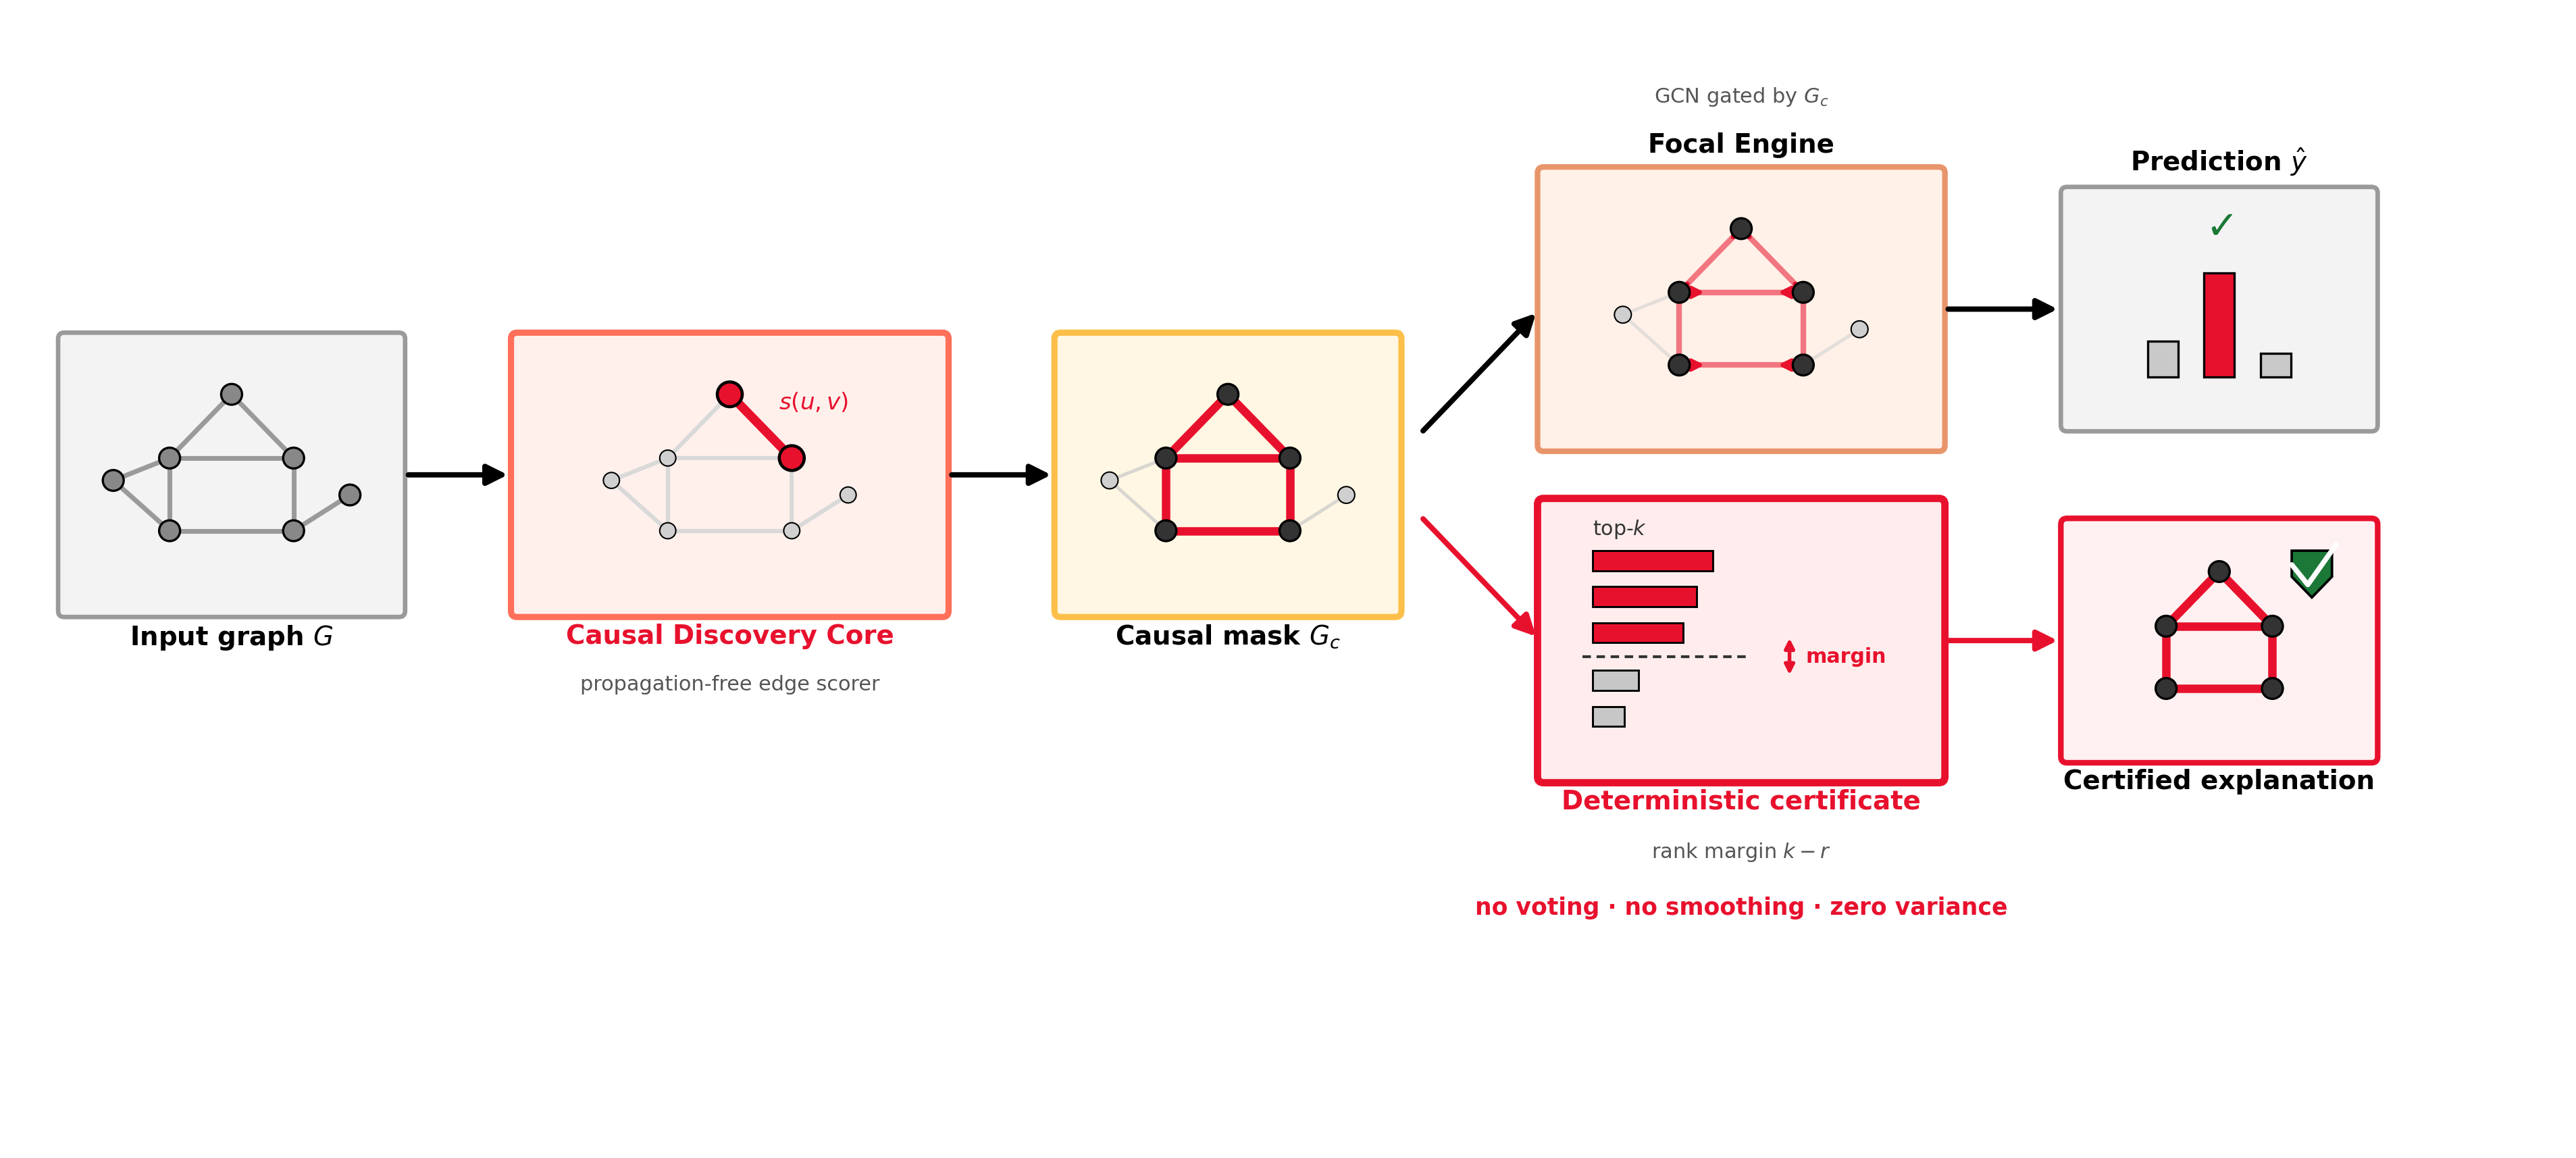
\includegraphics[width=\linewidth]{../../figures/F0_architecture.png}
  \caption{The \aeth{} pipeline: a propagation-free causal core scores each edge
  from its endpoints alone, producing a mask that gates prediction and feeds a
  \emph{deterministic} rank-margin certificate ($k-r$)---no voting, no
  smoothing.}
  \label{fig:arch}
\end{figure}

\begin{figure}[t]\centering
  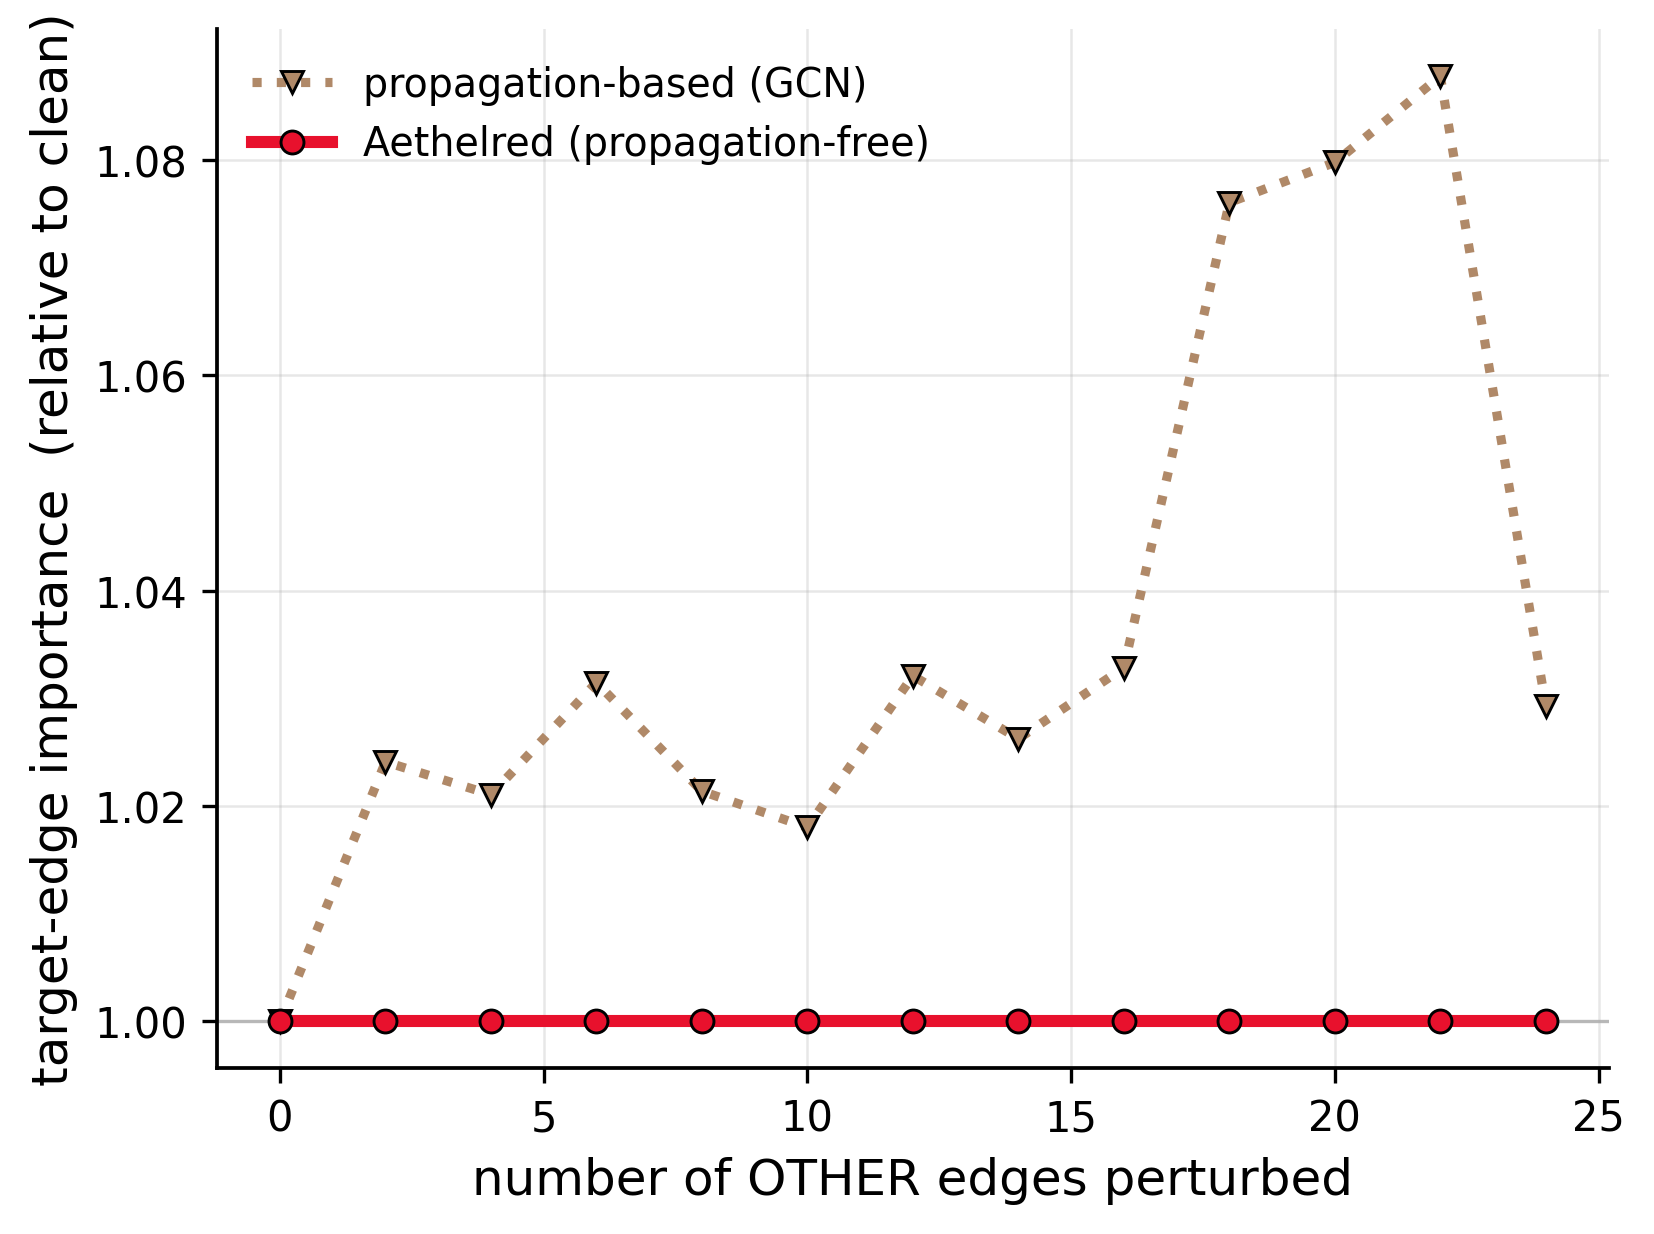
\includegraphics[width=0.82\linewidth]{../../figures/F10_edge_locality.png}
  \caption{Edge-locality. A target edge's importance vs.\ the number of
  \emph{other} edges perturbed: \aeth{}'s score is exactly invariant; a
  propagation-based (GCN) score drifts.}
  \label{fig:locality}
\end{figure}

\begin{figure}[t]\centering
  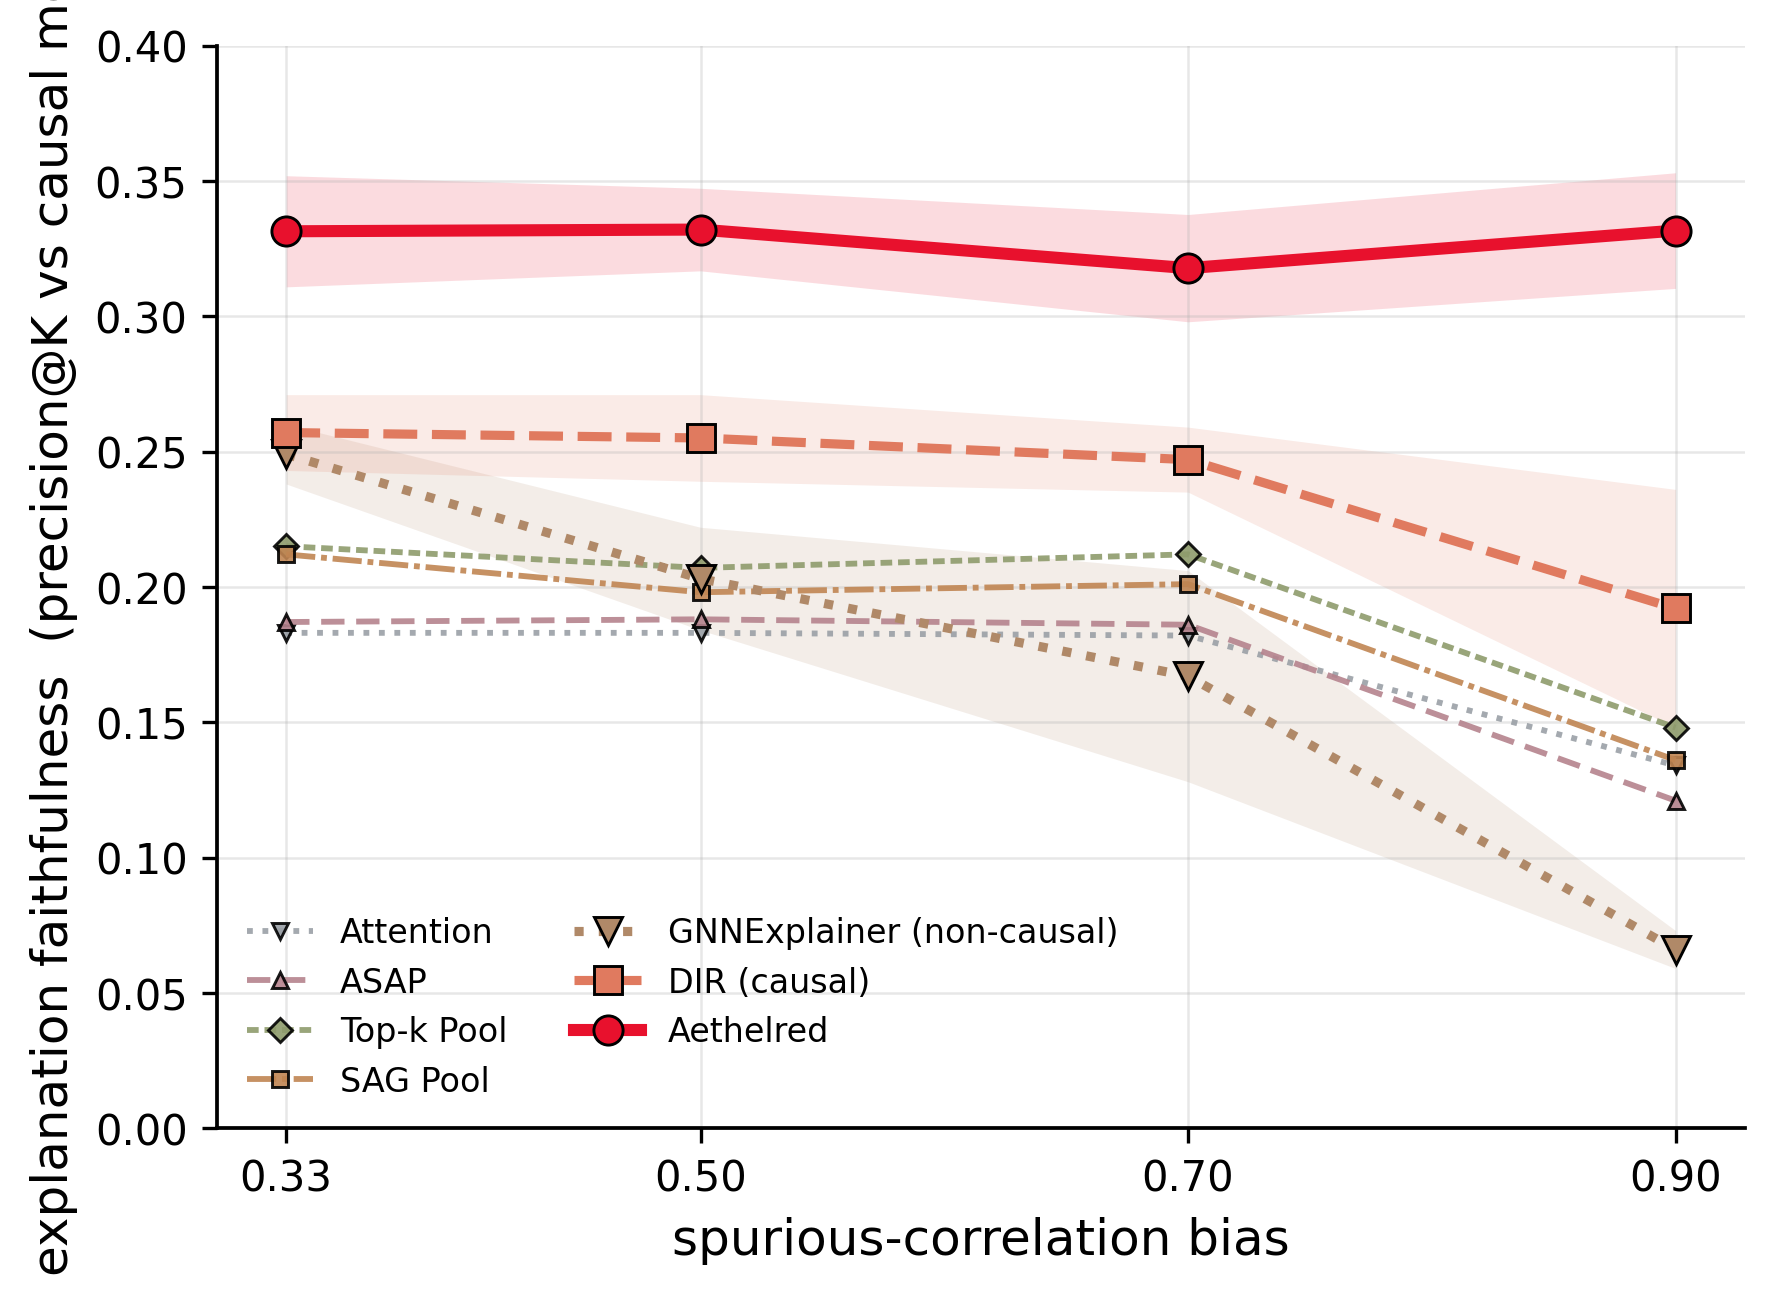
\includegraphics[width=0.9\linewidth]{../../figures/F9_spmotif_causal_vs_spurious.png}
  \caption{Faithfulness (precision@$K$ vs.\ the \emph{causal} motif) as spurious
  correlation strengthens on \textsc{SPMotif}. GNNExplainer and the pooling
  rationale baselines (Attention/ASAP/Top-k/SAG, DIR Table~2) collapse, DIR
  partly resists; \aeth{} is bias-invariant.}
  \label{fig:thesis}
\end{figure}

\begin{figure}[t]\centering
  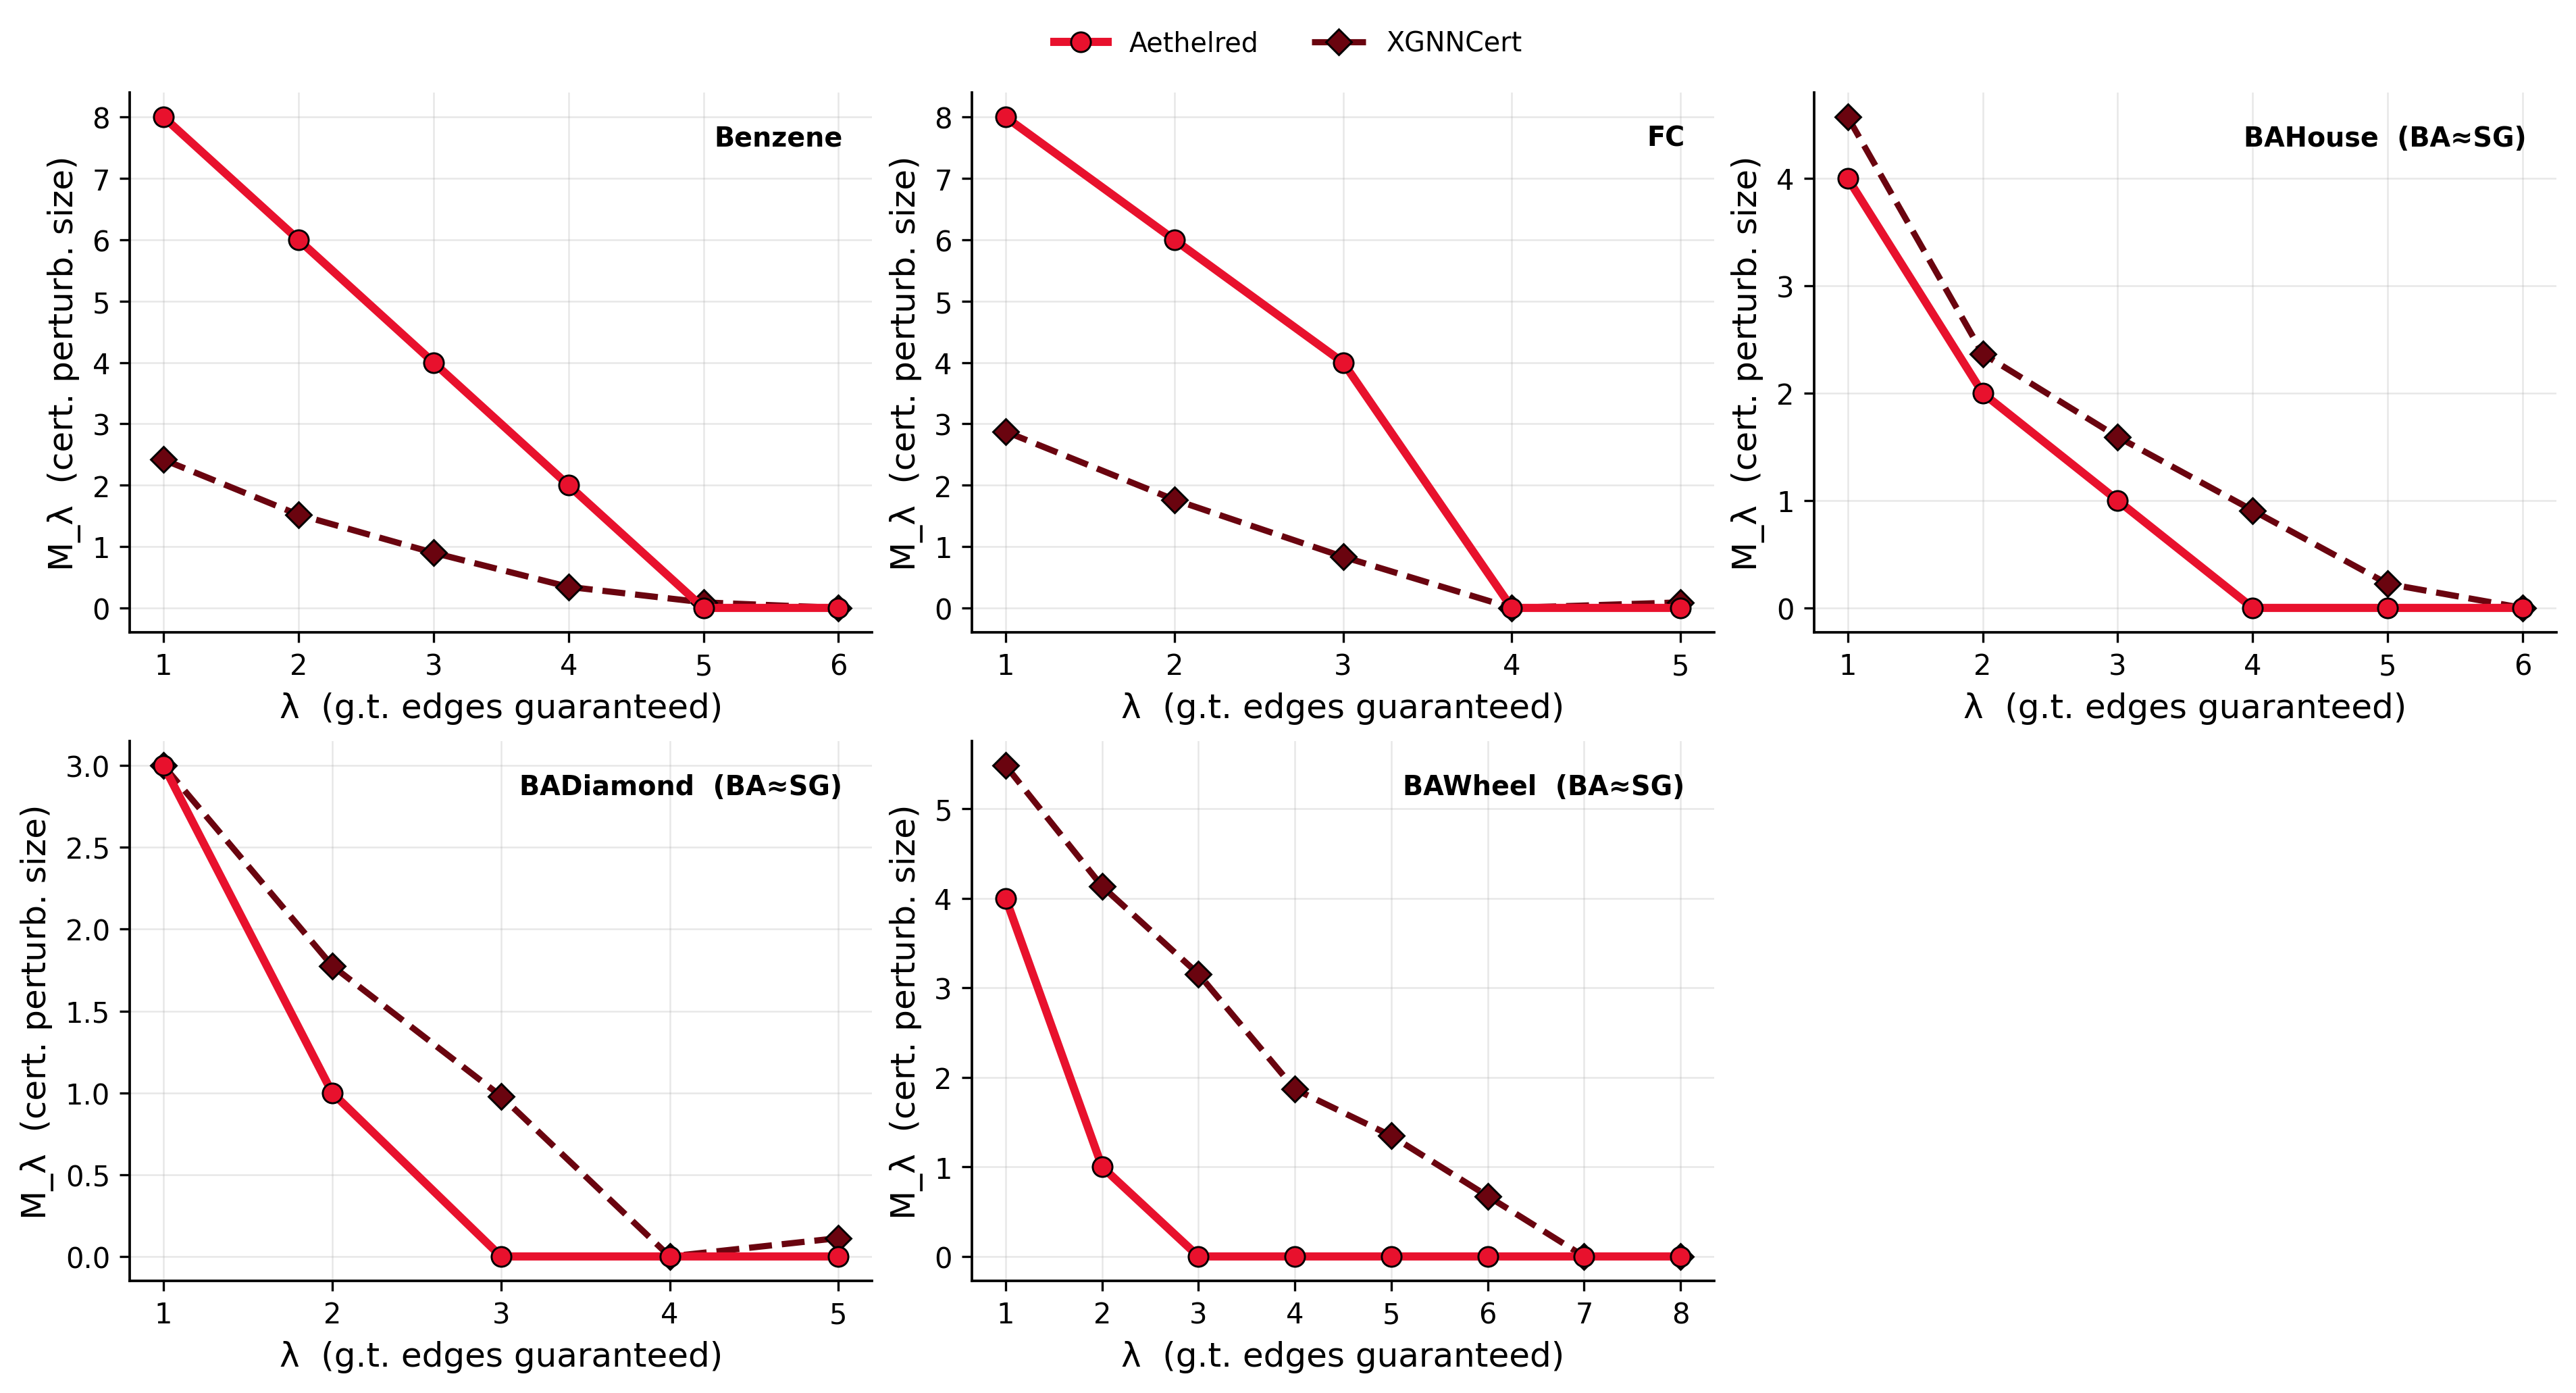
\includegraphics[width=\linewidth]{../../figures/F7_Mlambda_vs_lambda.png}
  \caption{Certified perturbation size $M_\lambda$ vs.\ guaranteed ground-truth
  edges $\lambda$ (\xgn{}'s own metric). \aeth{} vs.\ \xgn{}'s authoritative
  published default ($T{=}70$, PGExplainer).}
  \label{fig:mlambda}
\end{figure}

\begin{figure}[t]\centering
  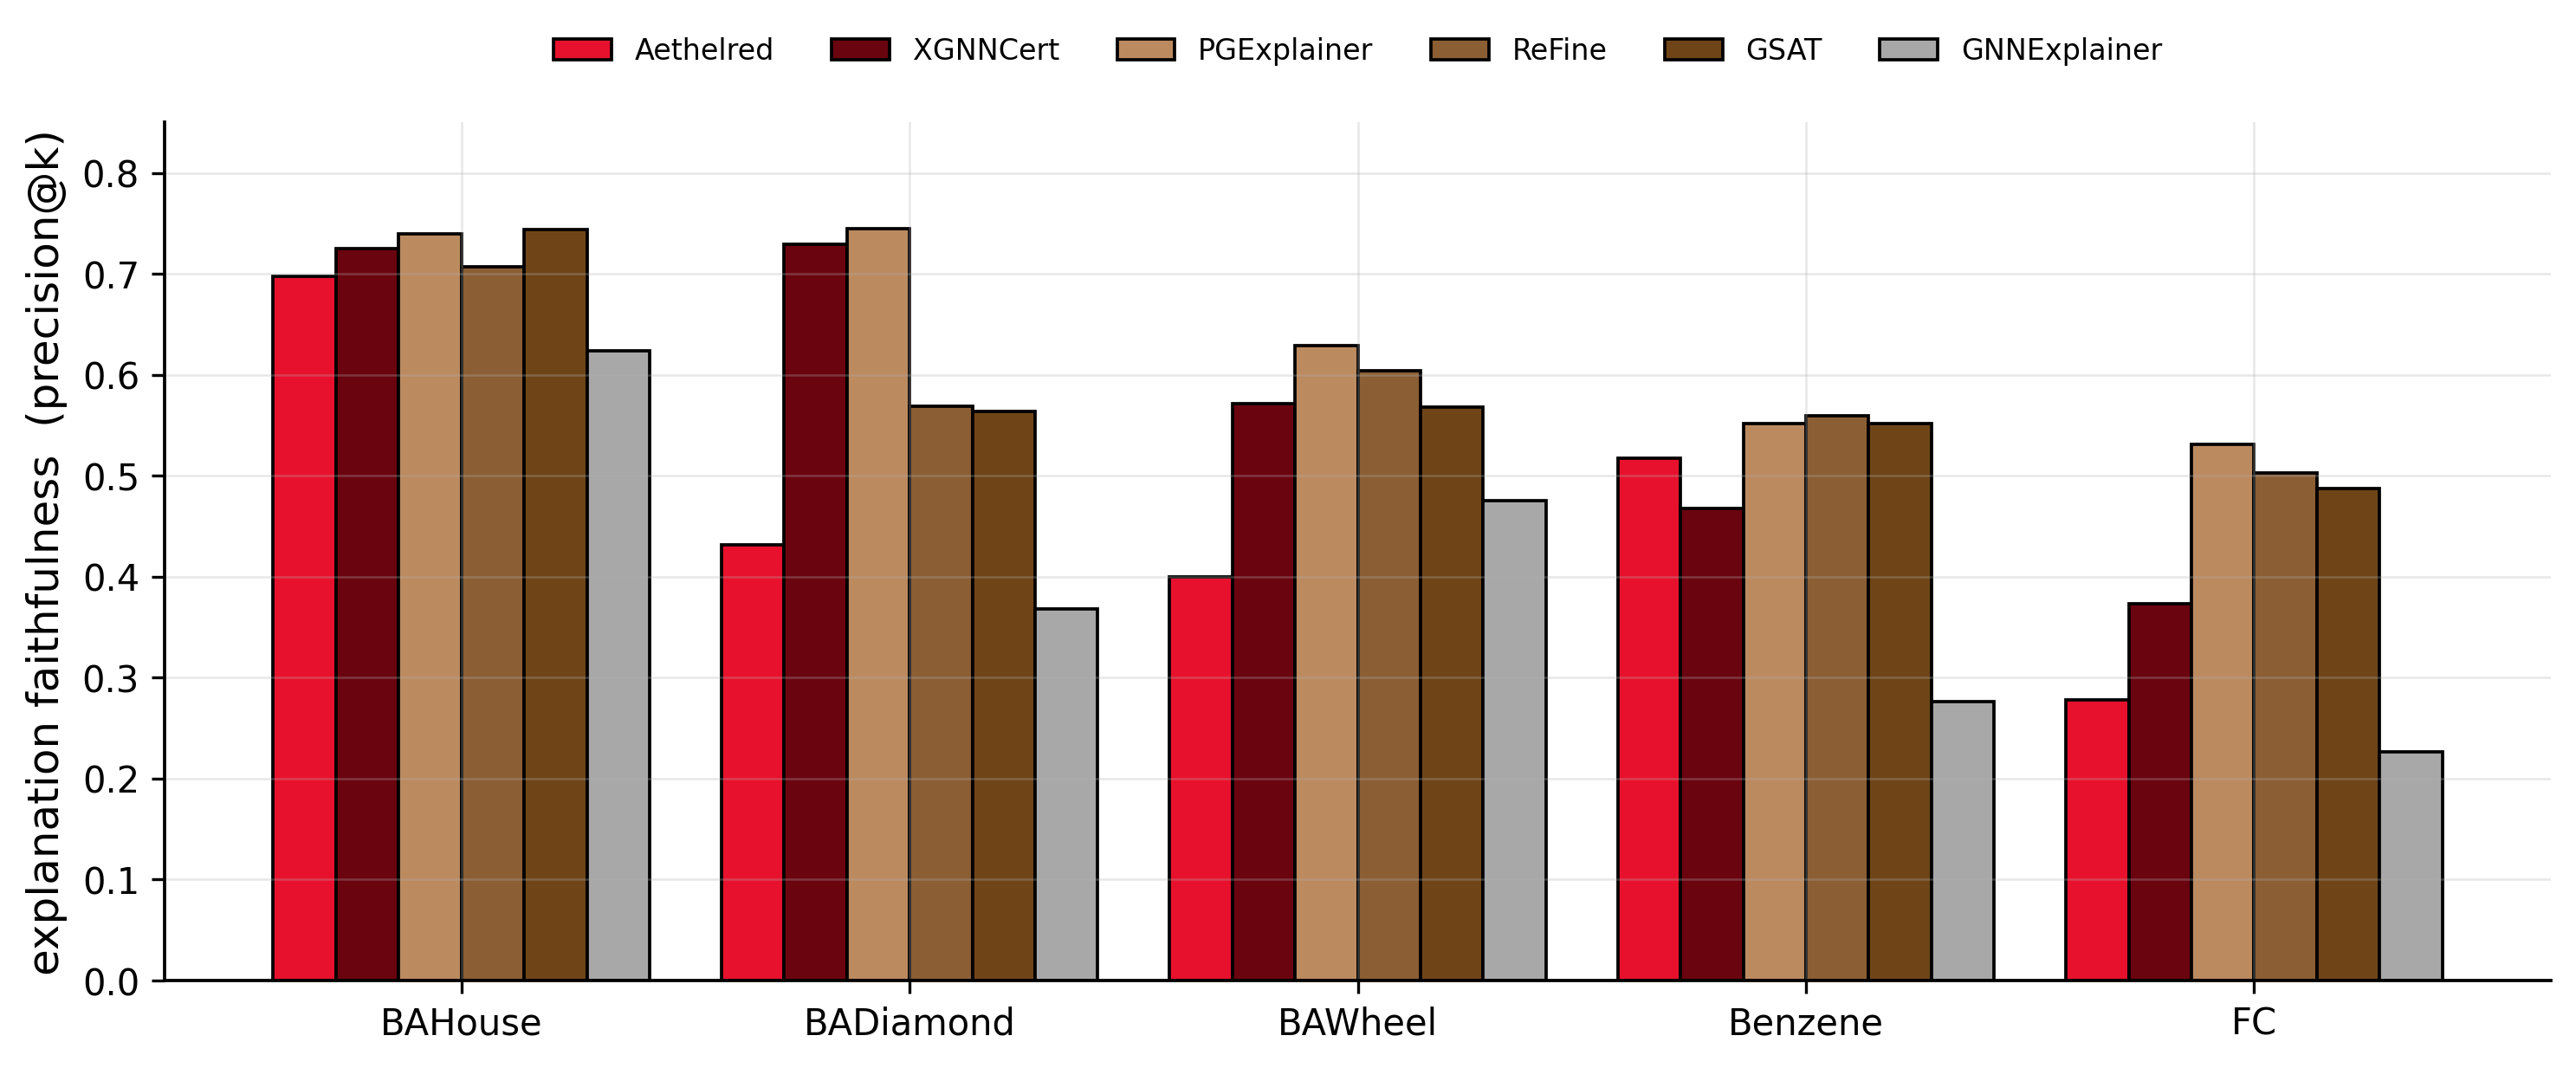
\includegraphics[width=\linewidth]{../../figures/F2c_unified_faithfulness.png}
  \caption{Clean explanation faithfulness: \aeth{} against all explanation
  baselines (\xgn{}, PGExplainer, ReFine, GSAT, GNNExplainer) on the five
  ground-truth-motif datasets.}
  \label{fig:unifaith}
\end{figure}

\begin{figure}[t]\centering
  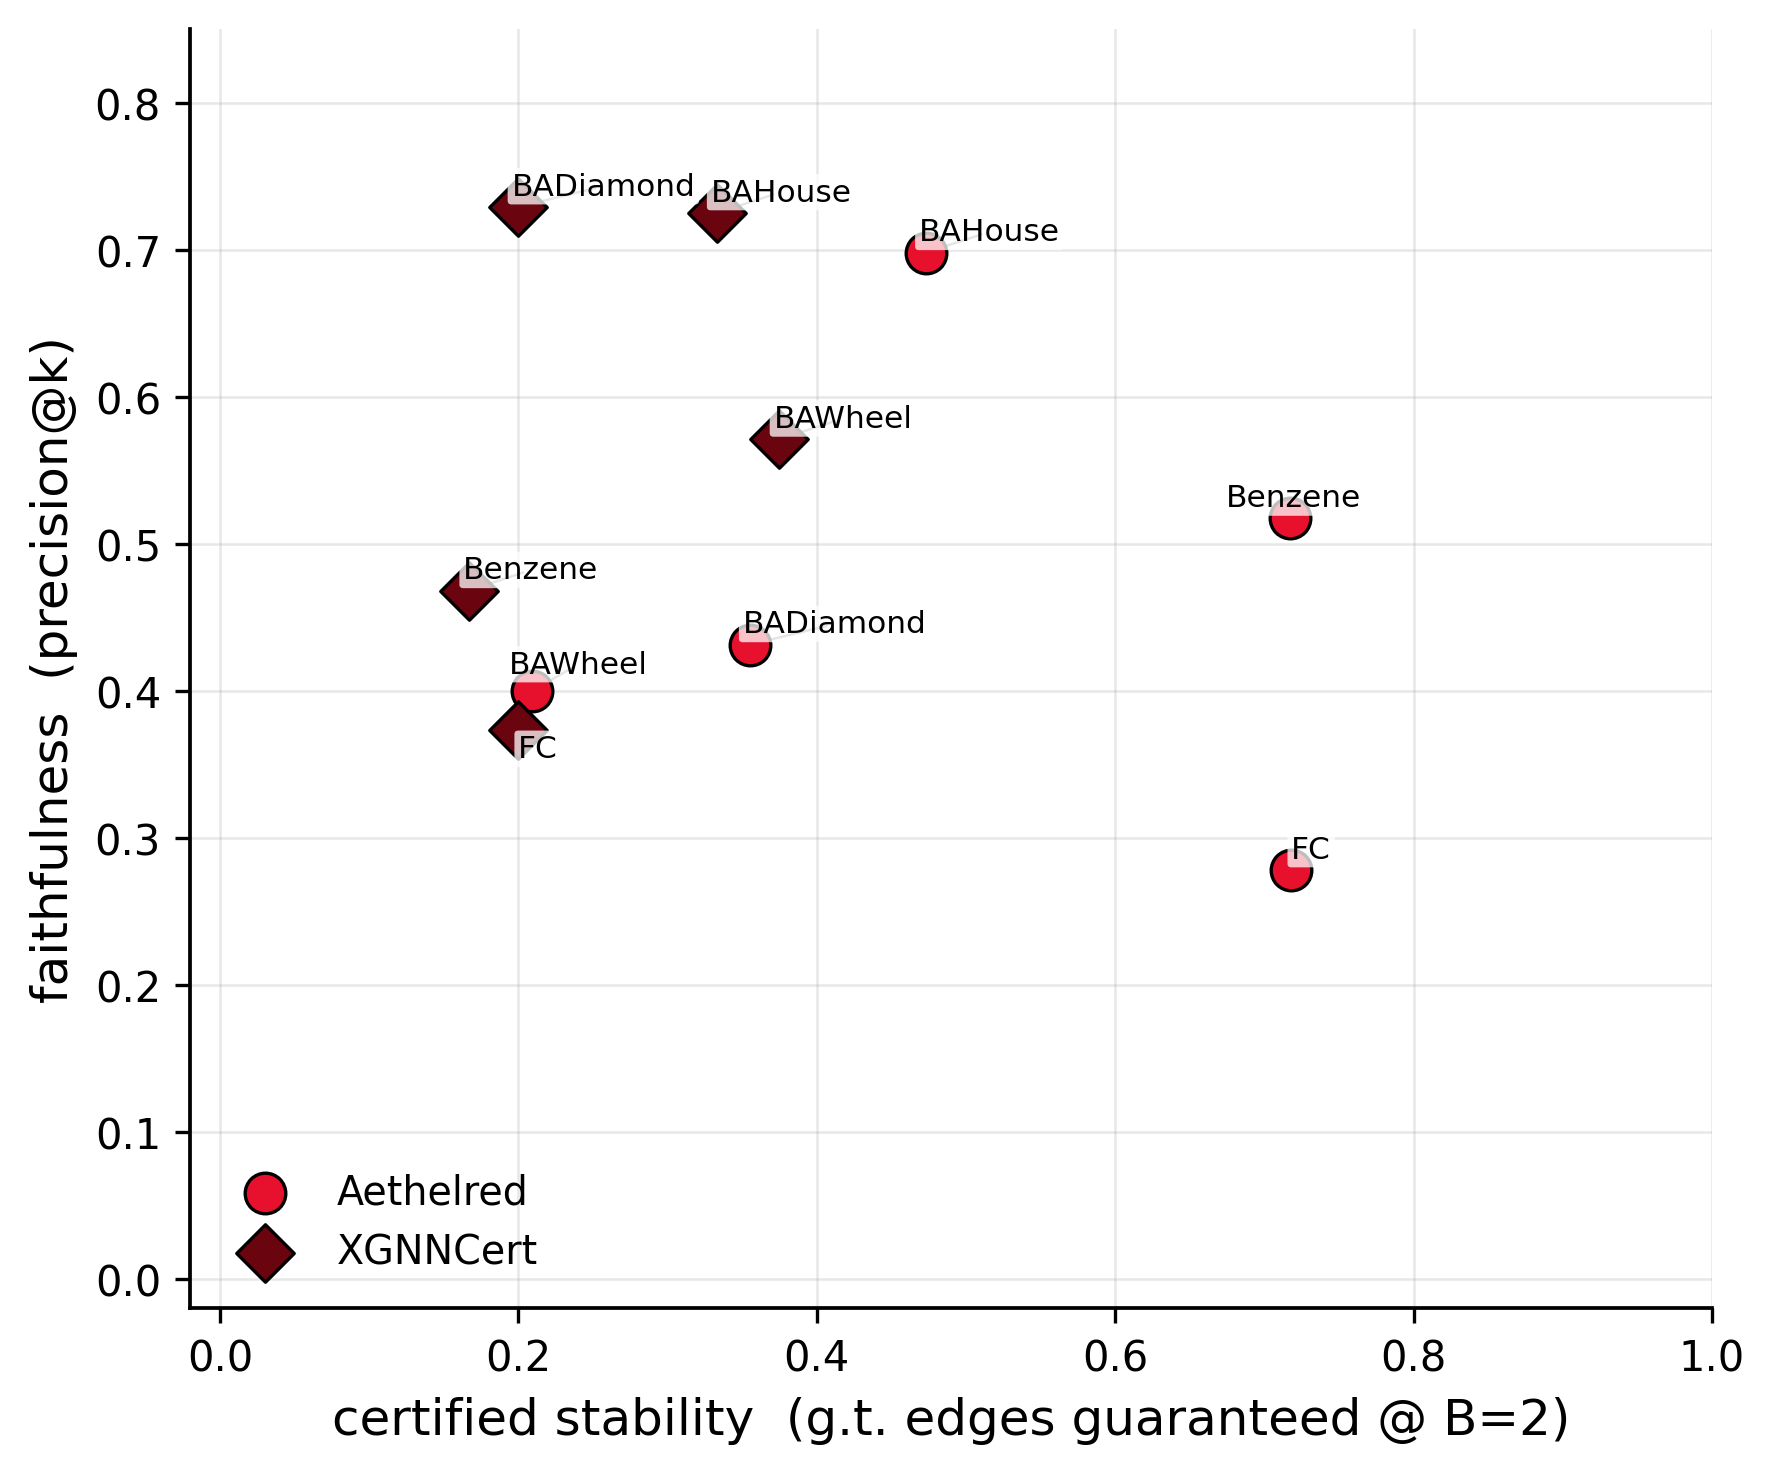
\includegraphics[width=0.85\linewidth]{../../figures/F3_faithfulness_stability_frontier.png}
  \caption{Faithfulness vs.\ certified stability (ground-truth edges guaranteed at
  $B{=}2$). Top-right is best; \xgn{} from published values.}
  \label{fig:frontier}
\end{figure}

\begin{figure}[t]\centering
  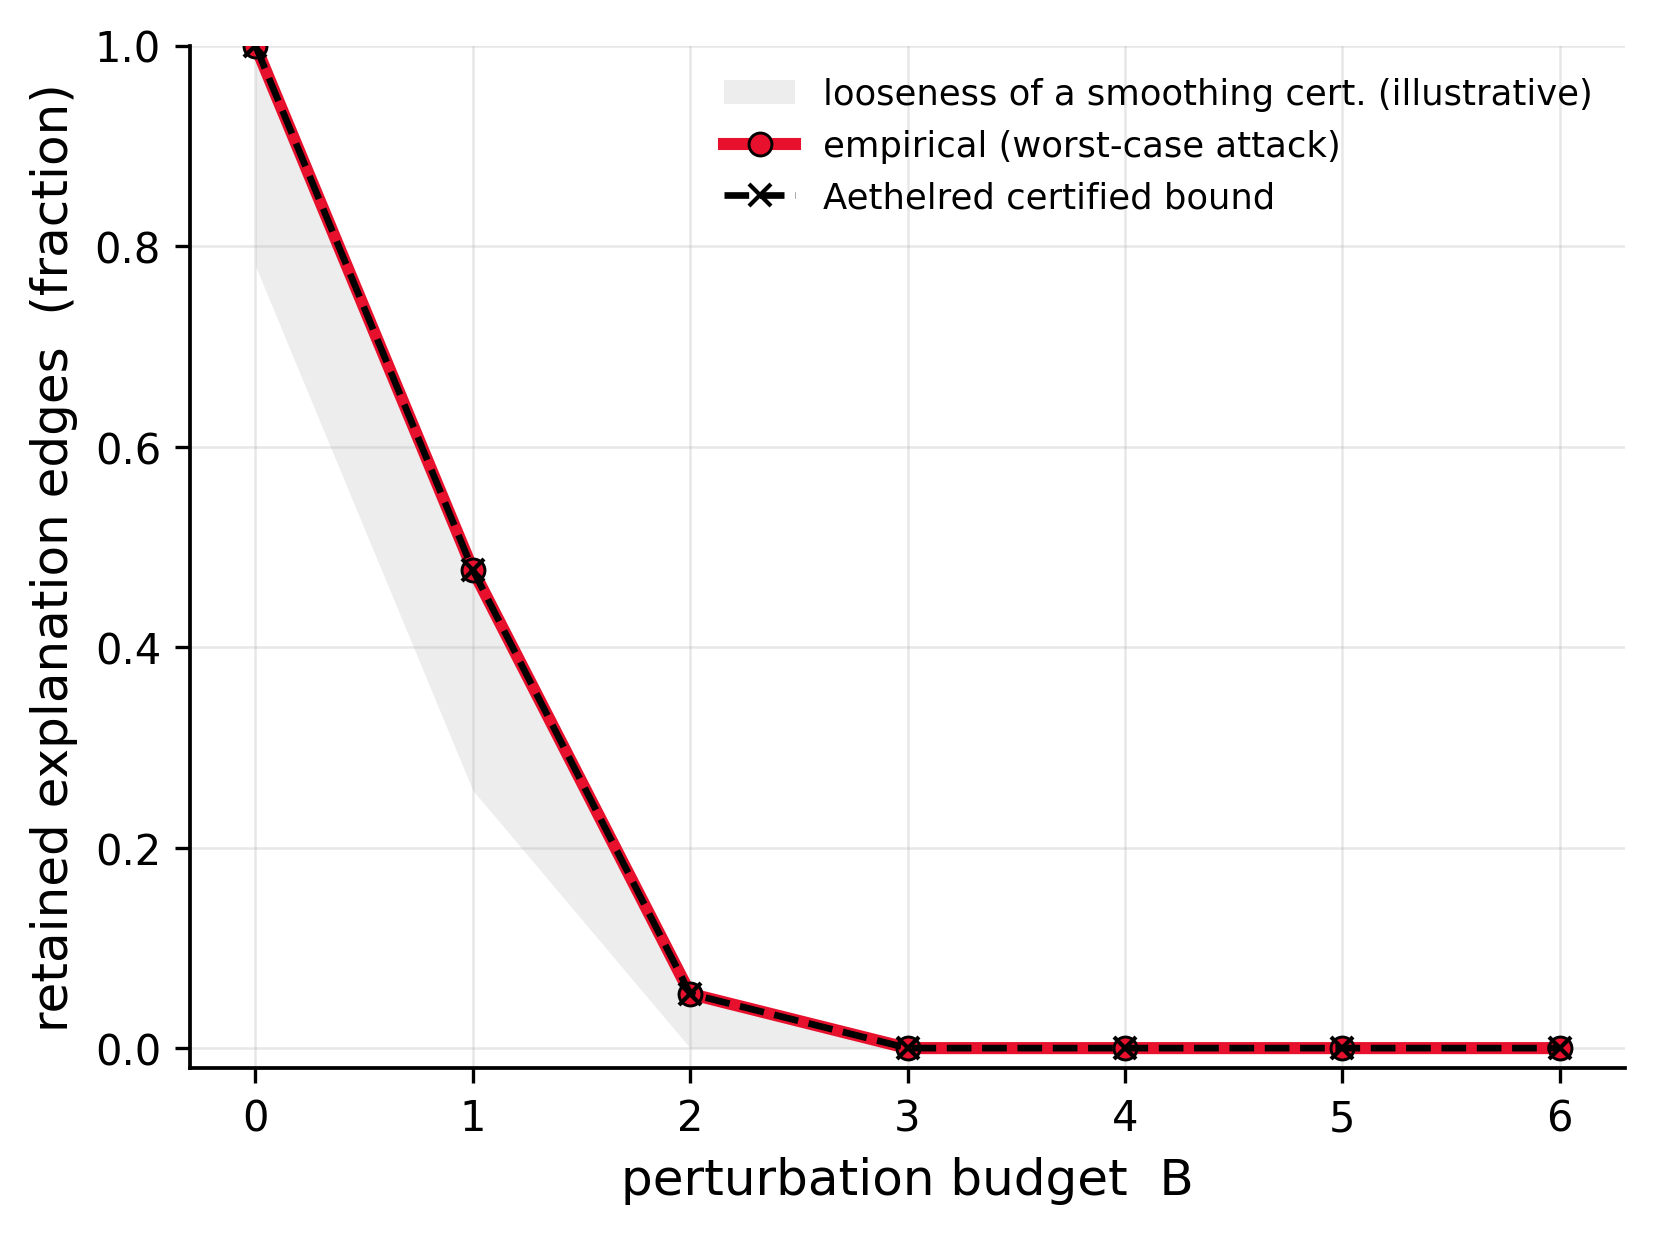
\includegraphics[width=0.82\linewidth]{../../figures/F11_certificate_tightness.png}
  \caption{Tightness: \aeth{}'s certified bound coincides with the empirical
  worst-case (gap $=0$); the grey band marks a smoothing certificate's looseness.}
  \label{fig:tight}
\end{figure}

\begin{figure}[t]\centering
  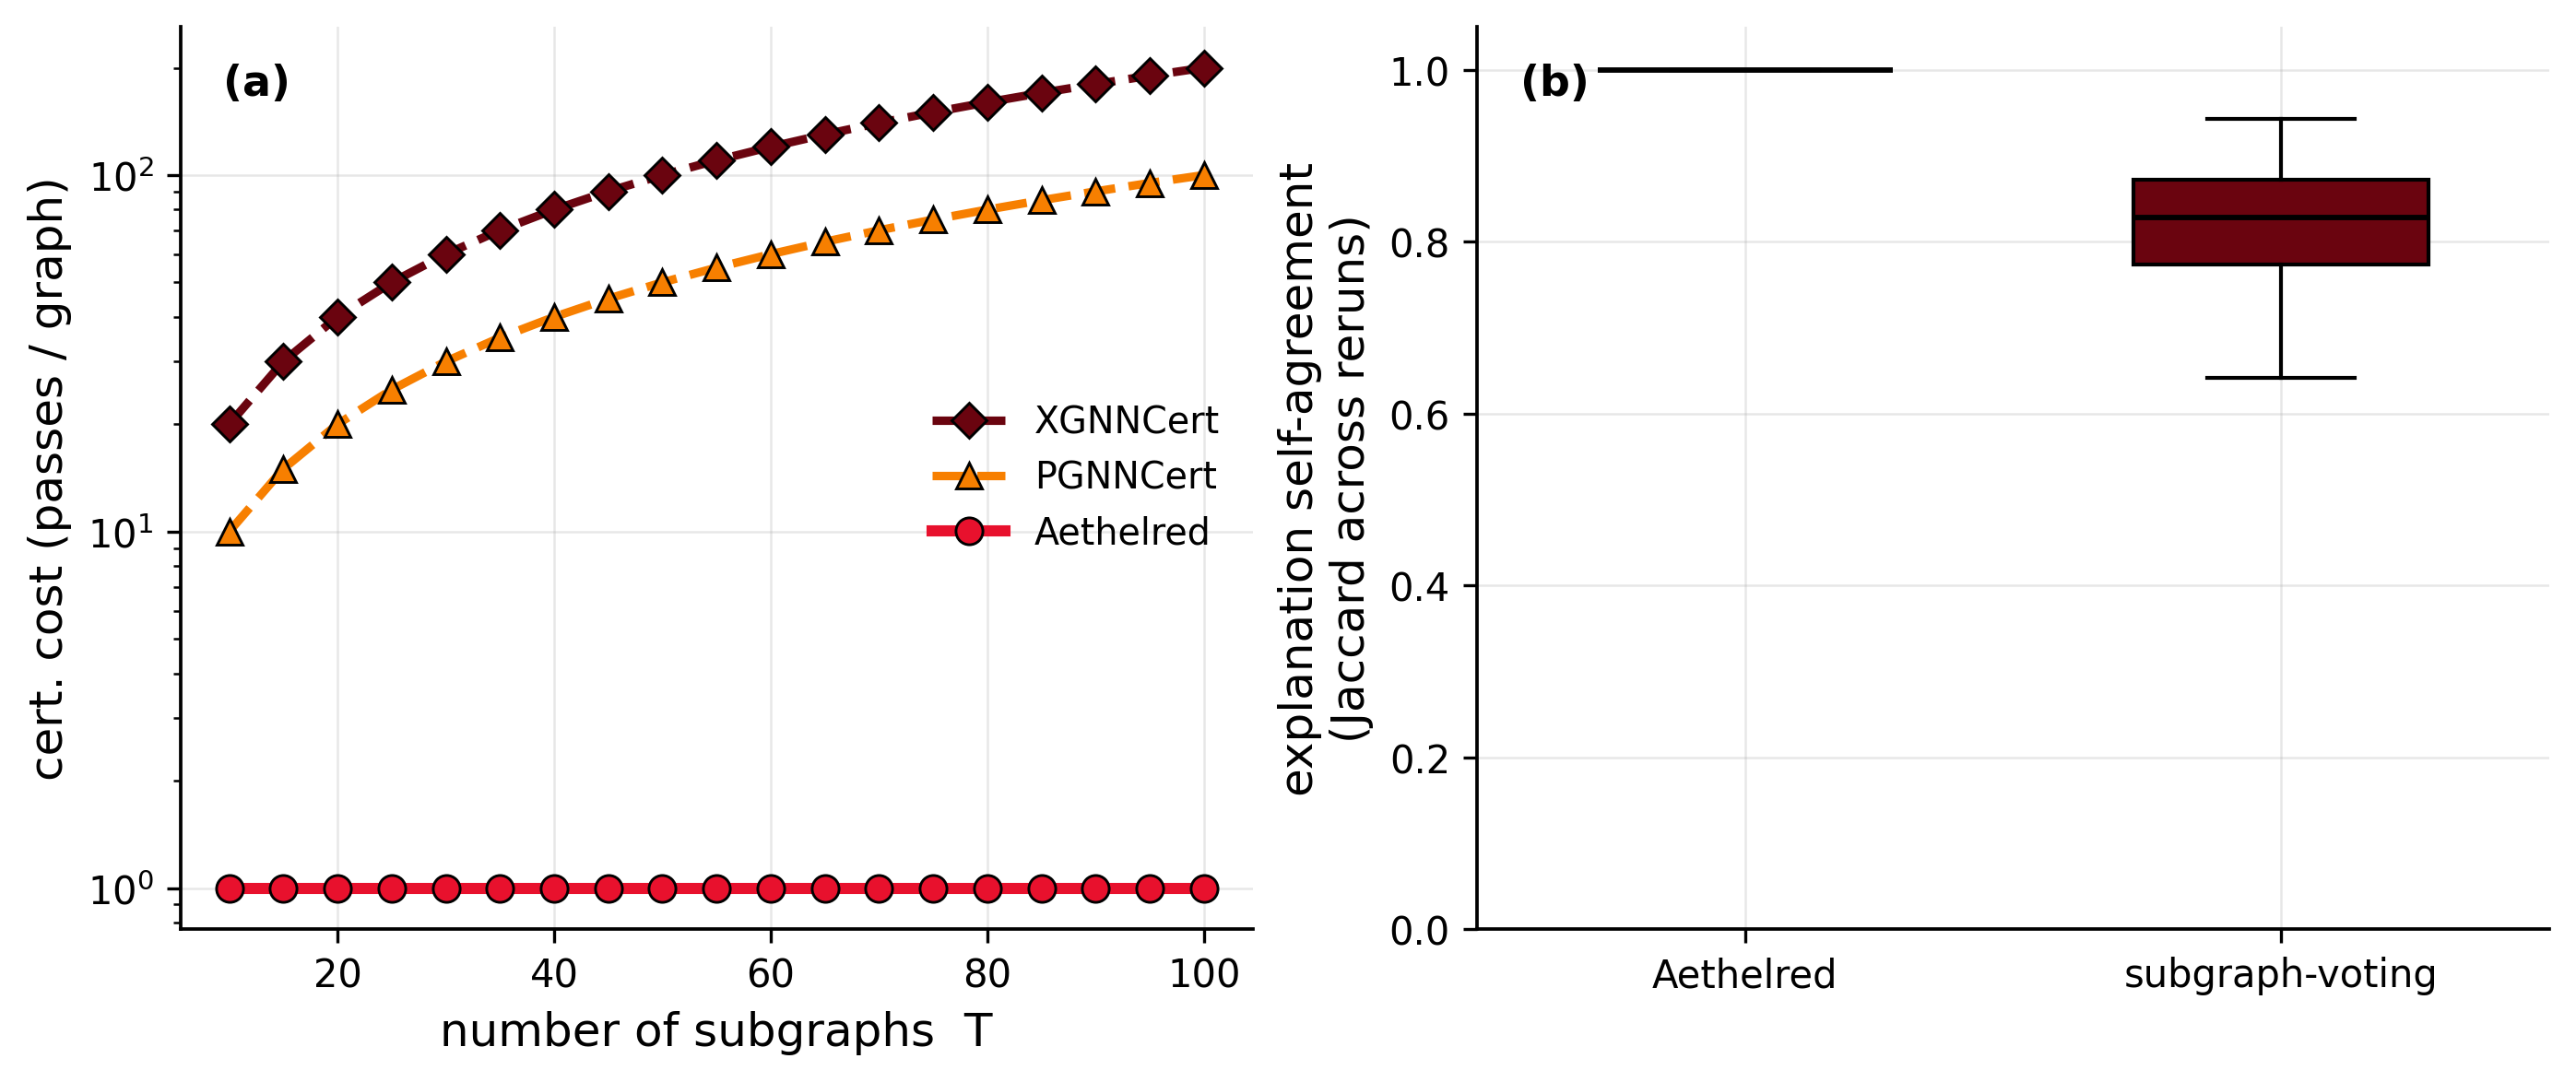
\includegraphics[width=\linewidth]{../../figures/F56_efficiency_determinism.png}
  \caption{(a) Certification cost vs.\ \#sub-graphs $T$ (log scale).
  (b) Explanation self-agreement across reruns.}
  \label{fig:eff}
\end{figure}

\begin{figure}[t]\centering
  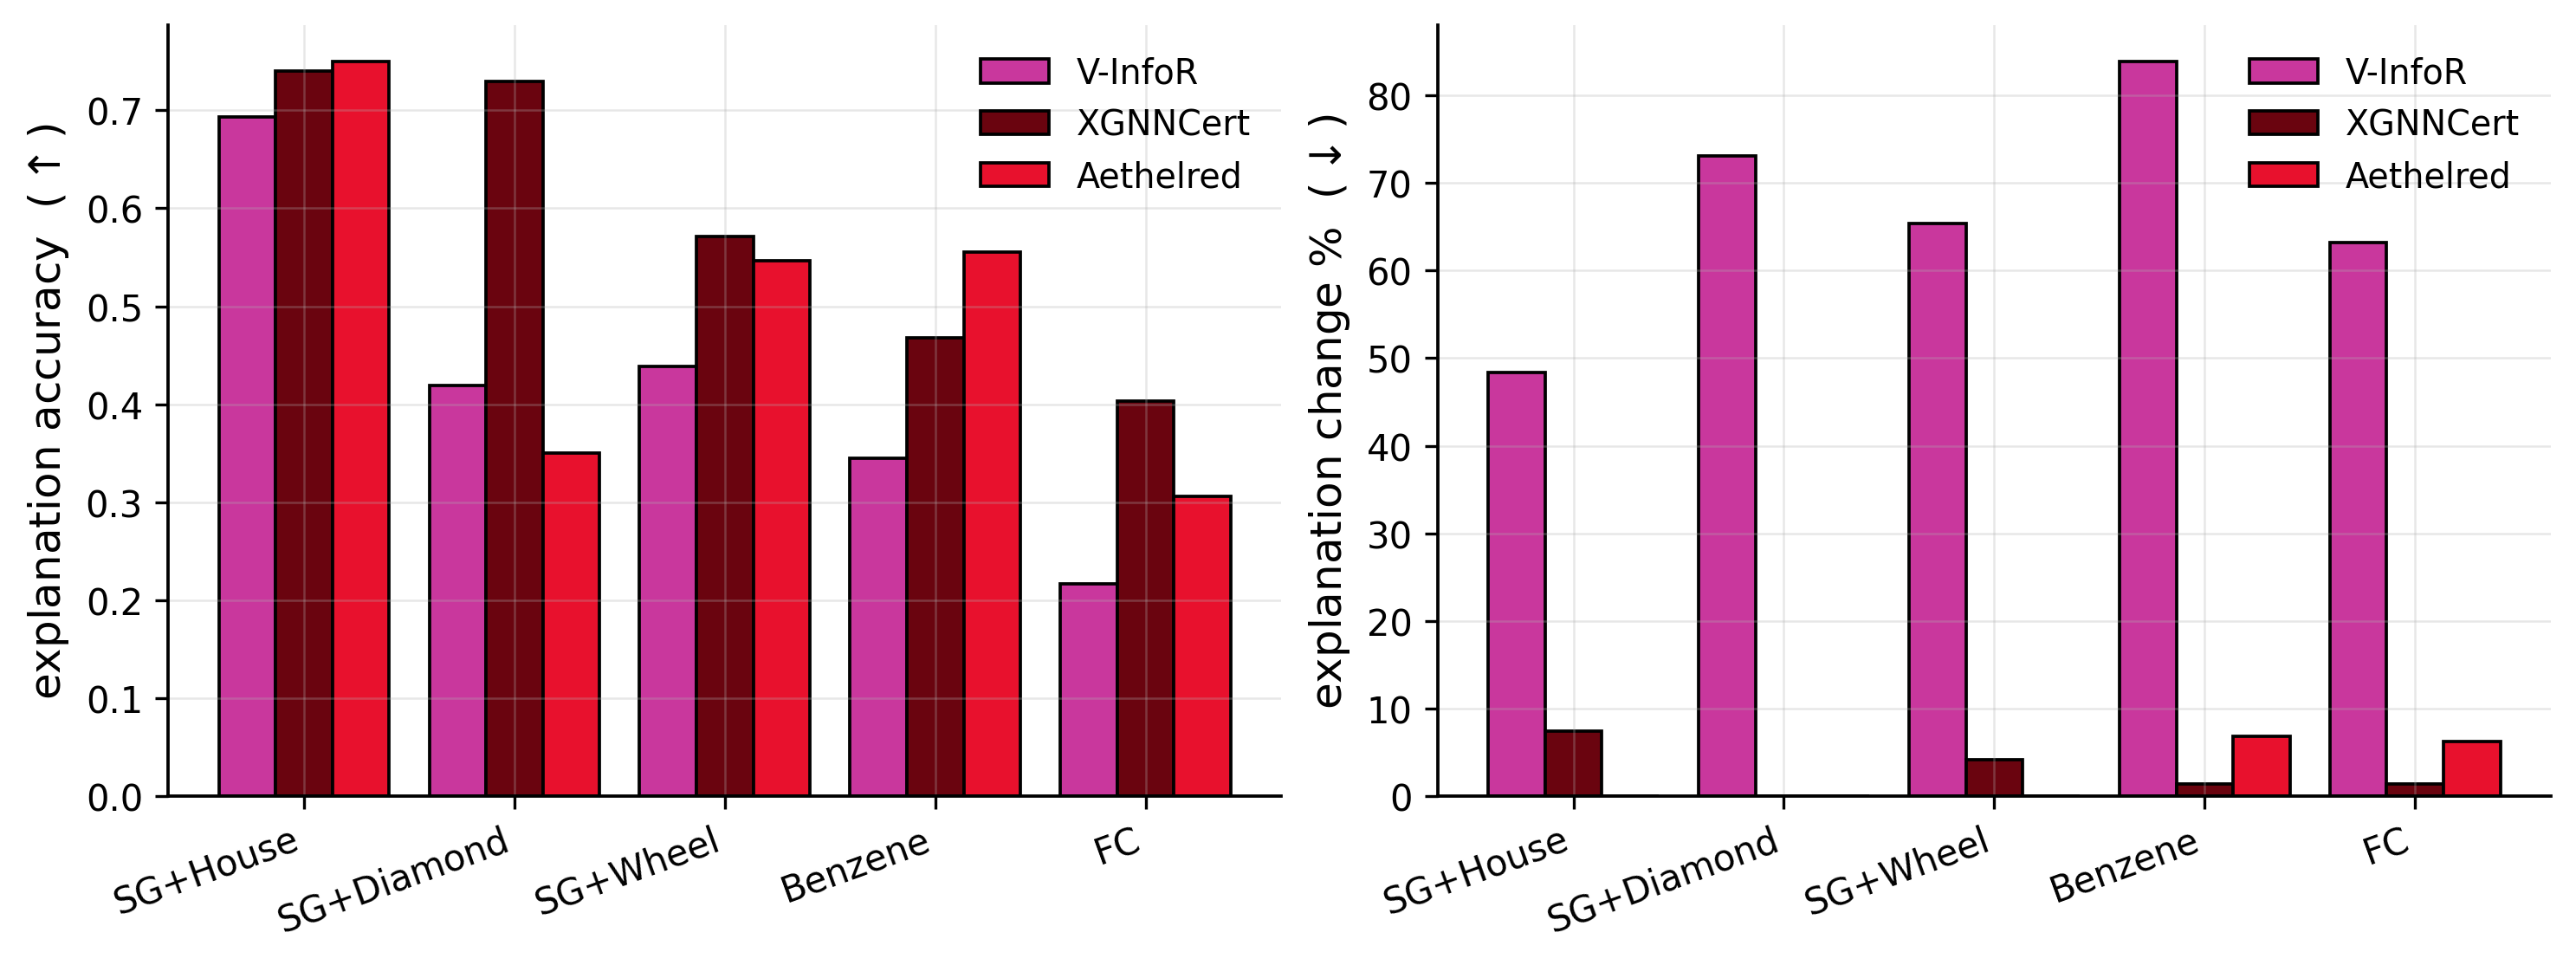
\includegraphics[width=\linewidth]{../../figures/F2b_explanation_robustness_vs_VInfoR.png}
  \caption{Explanation robustness under a $2$-edge attack: faithfulness
  ($\uparrow$) and drift ($\downarrow$) for \aeth{}, \xgn{}, and
  \textcolor{vinfomag}{V-InfoR}.}
  \label{fig:attack}
\end{figure}

\begin{figure}[t]\centering
  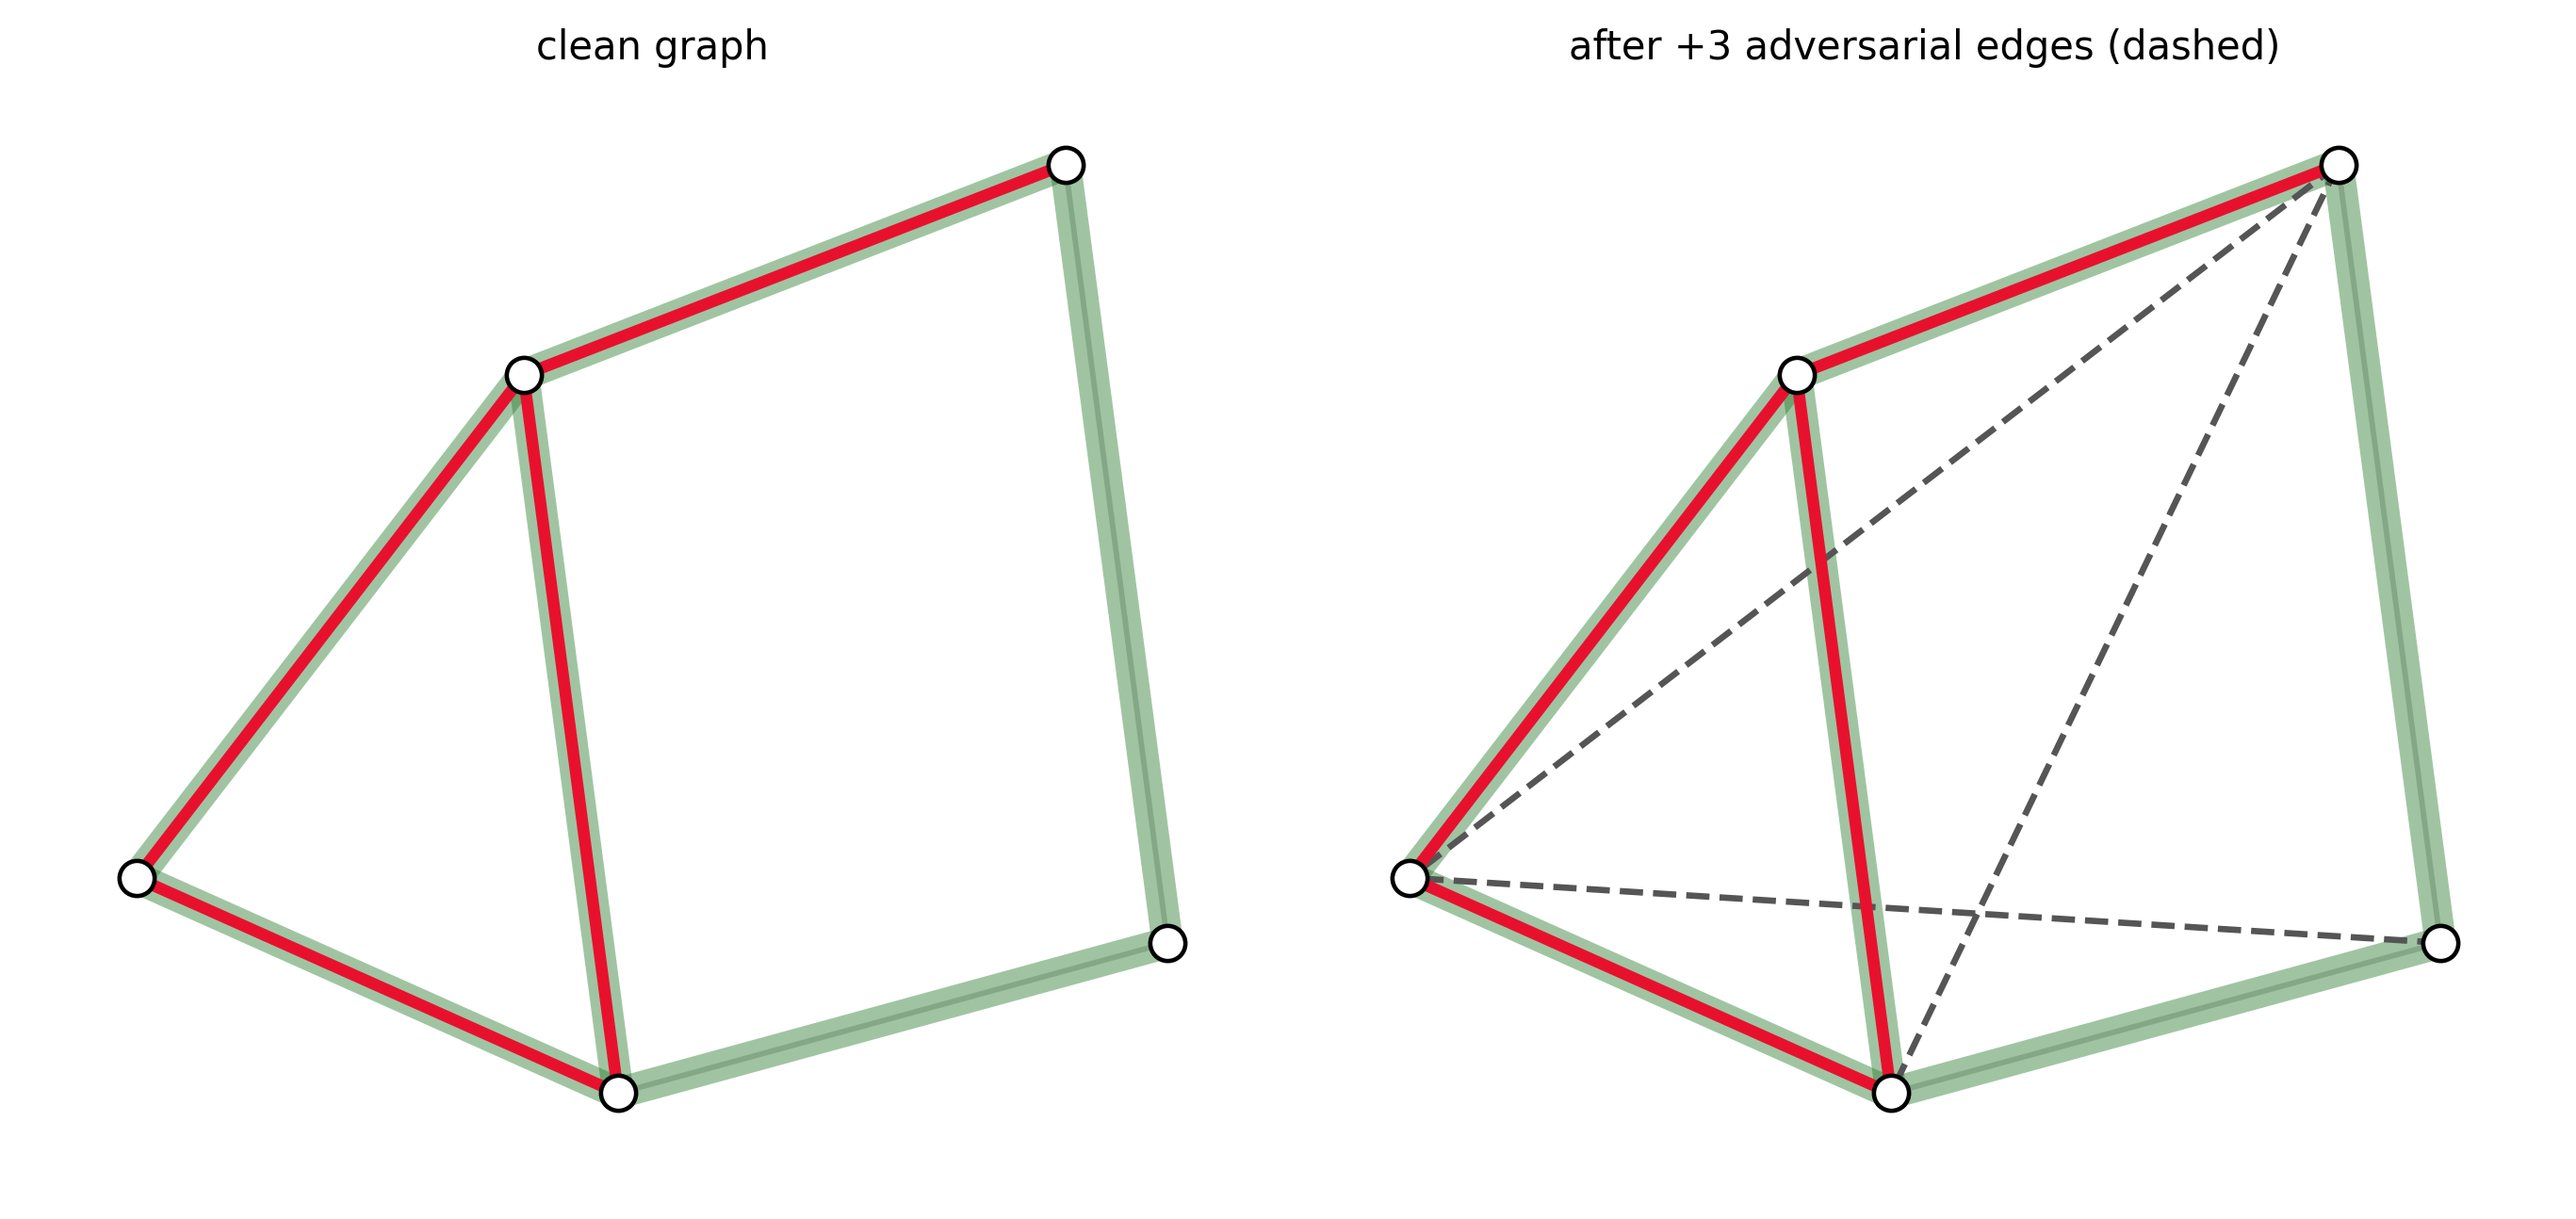
\includegraphics[width=\linewidth]{../../figures/F4_qualitative_explanation.png}
  \caption{\aeth{}'s certified explanation (red) on the ground-truth motif
  (green), before/after $3$ adversarial edges (dashed): the certified subset is
  unchanged.}
  \label{fig:qual}
\end{figure}

\begin{figure}[t]\centering
  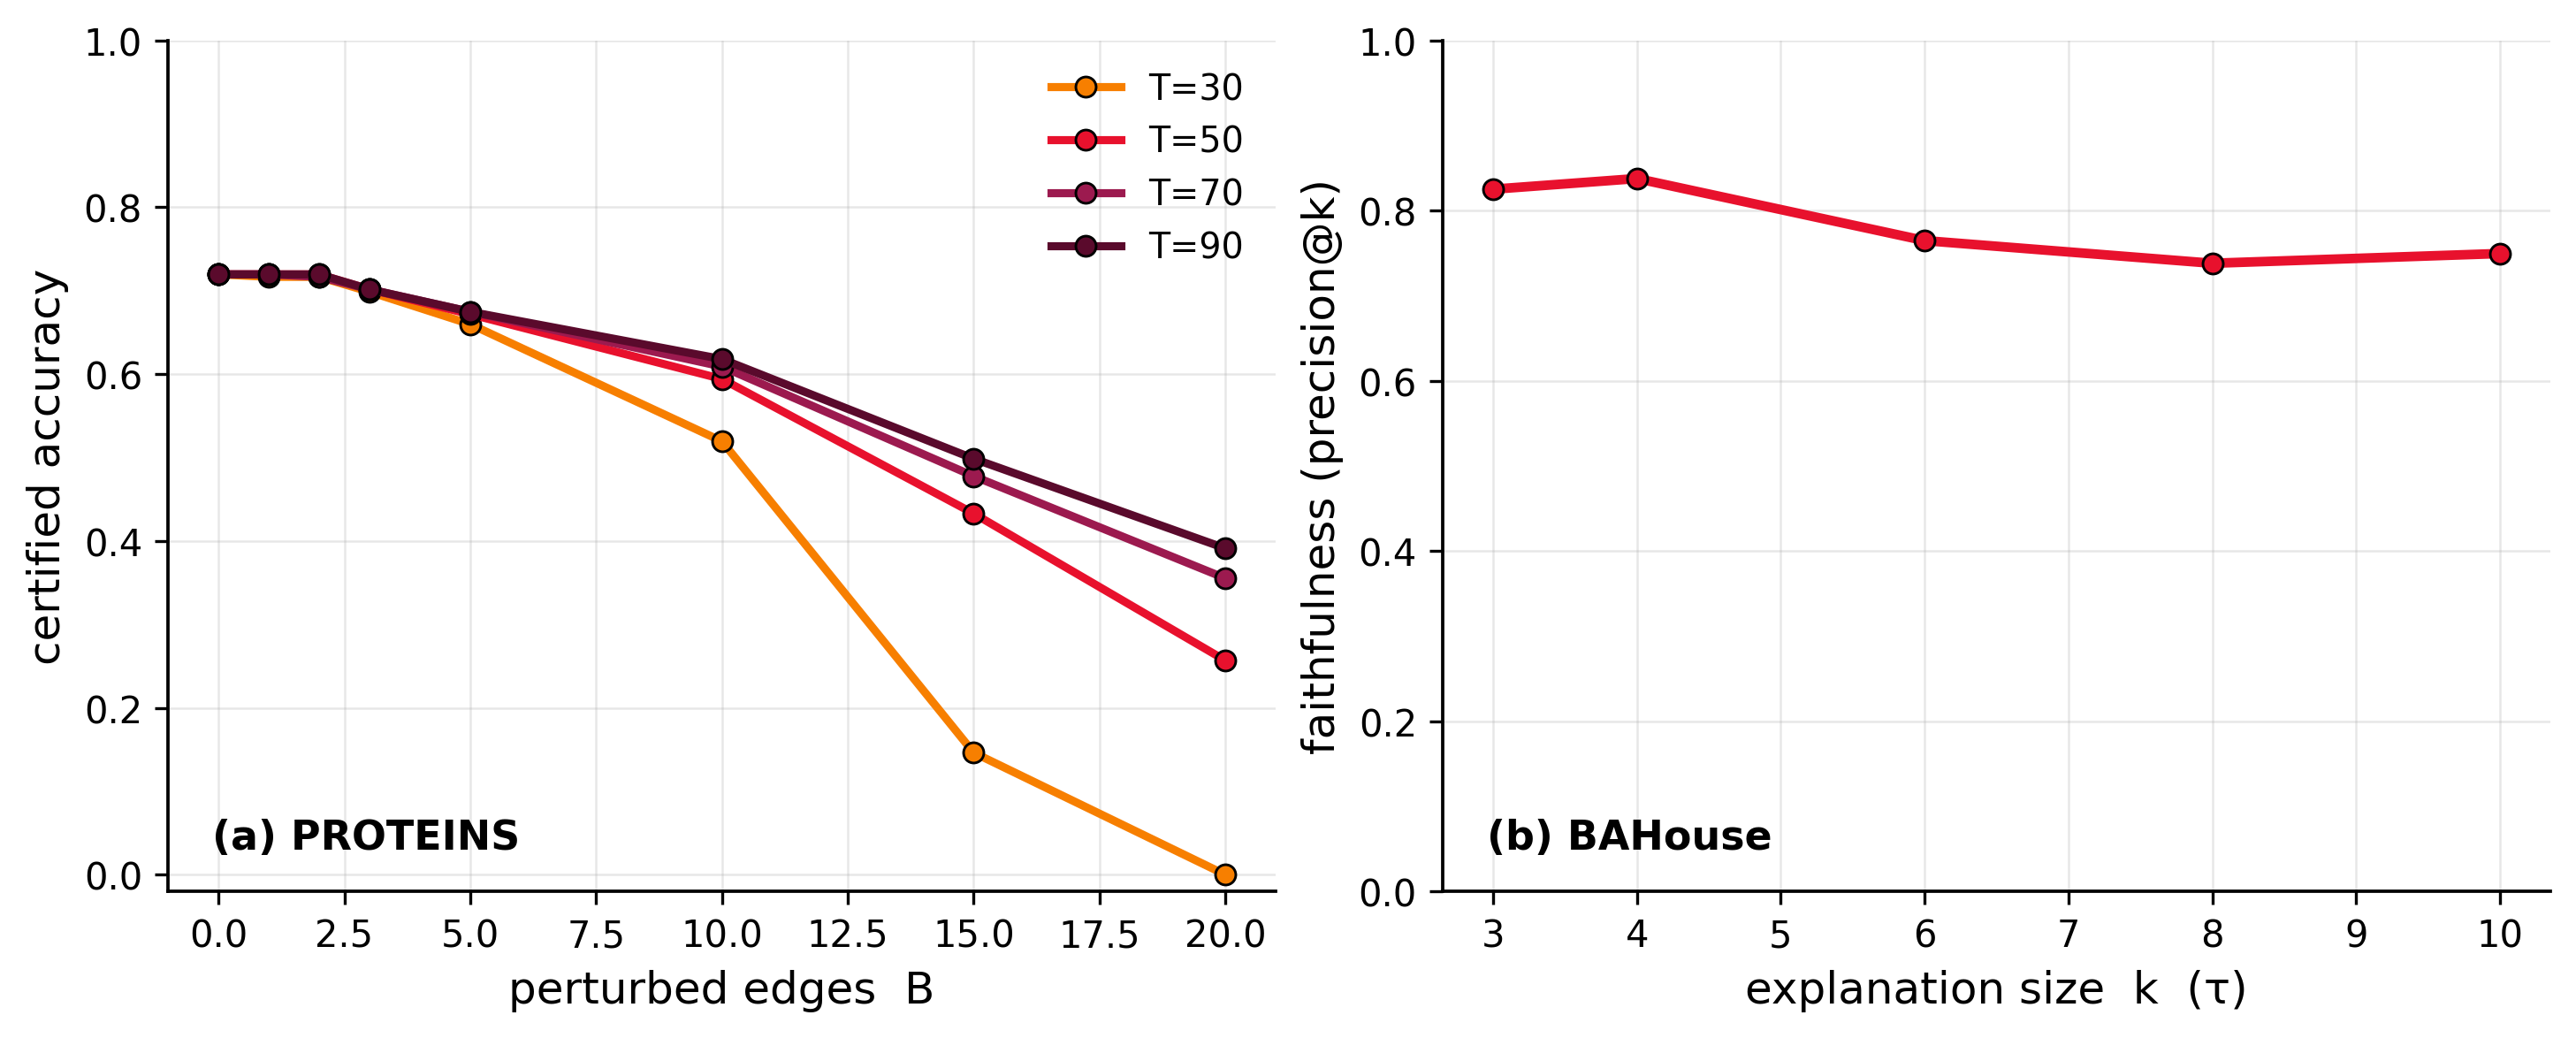
\includegraphics[width=\linewidth]{../../figures/F8_sensitivity.png}
  \caption{(a) Certified accuracy vs.\ budget for $T\!\in\!\{30,50,70,90\}$.
  (b) Faithfulness vs.\ explanation size $k$.}
  \label{fig:sens}
\end{figure}

\begin{figure}[t]\centering
  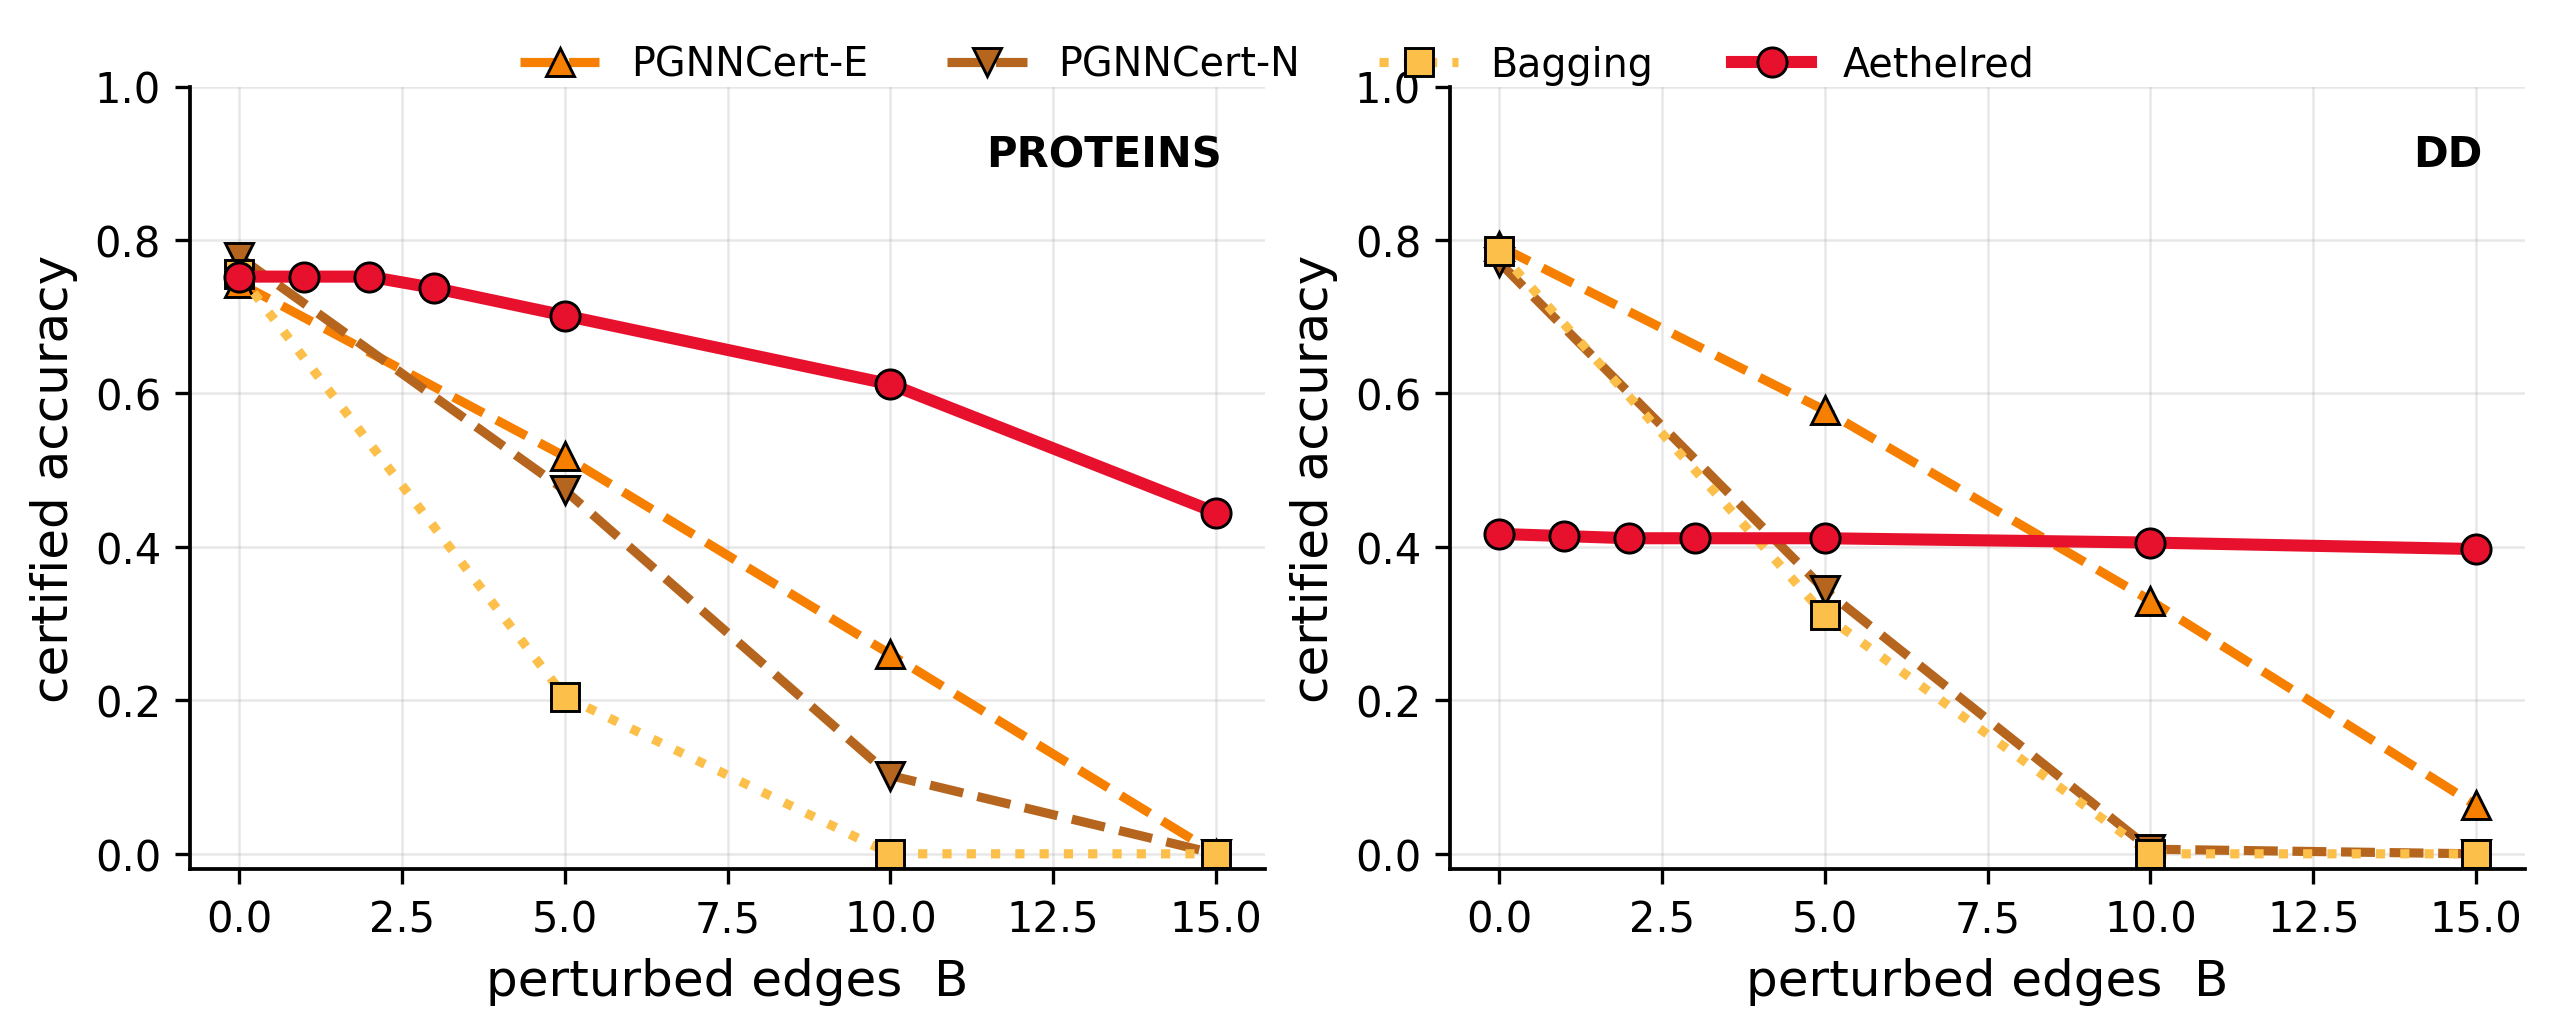
\includegraphics[width=\linewidth]{../../figures/F1_certified_prediction_vs_budget.png}
  \caption{Certified \emph{prediction} accuracy vs.\ edge budget (secondary
  axis), PROTEINS/DD; baselines from \pgn{}'s Table~2.}
  \label{fig:predcert}
\end{figure}

\begin{figure}[t]\centering
  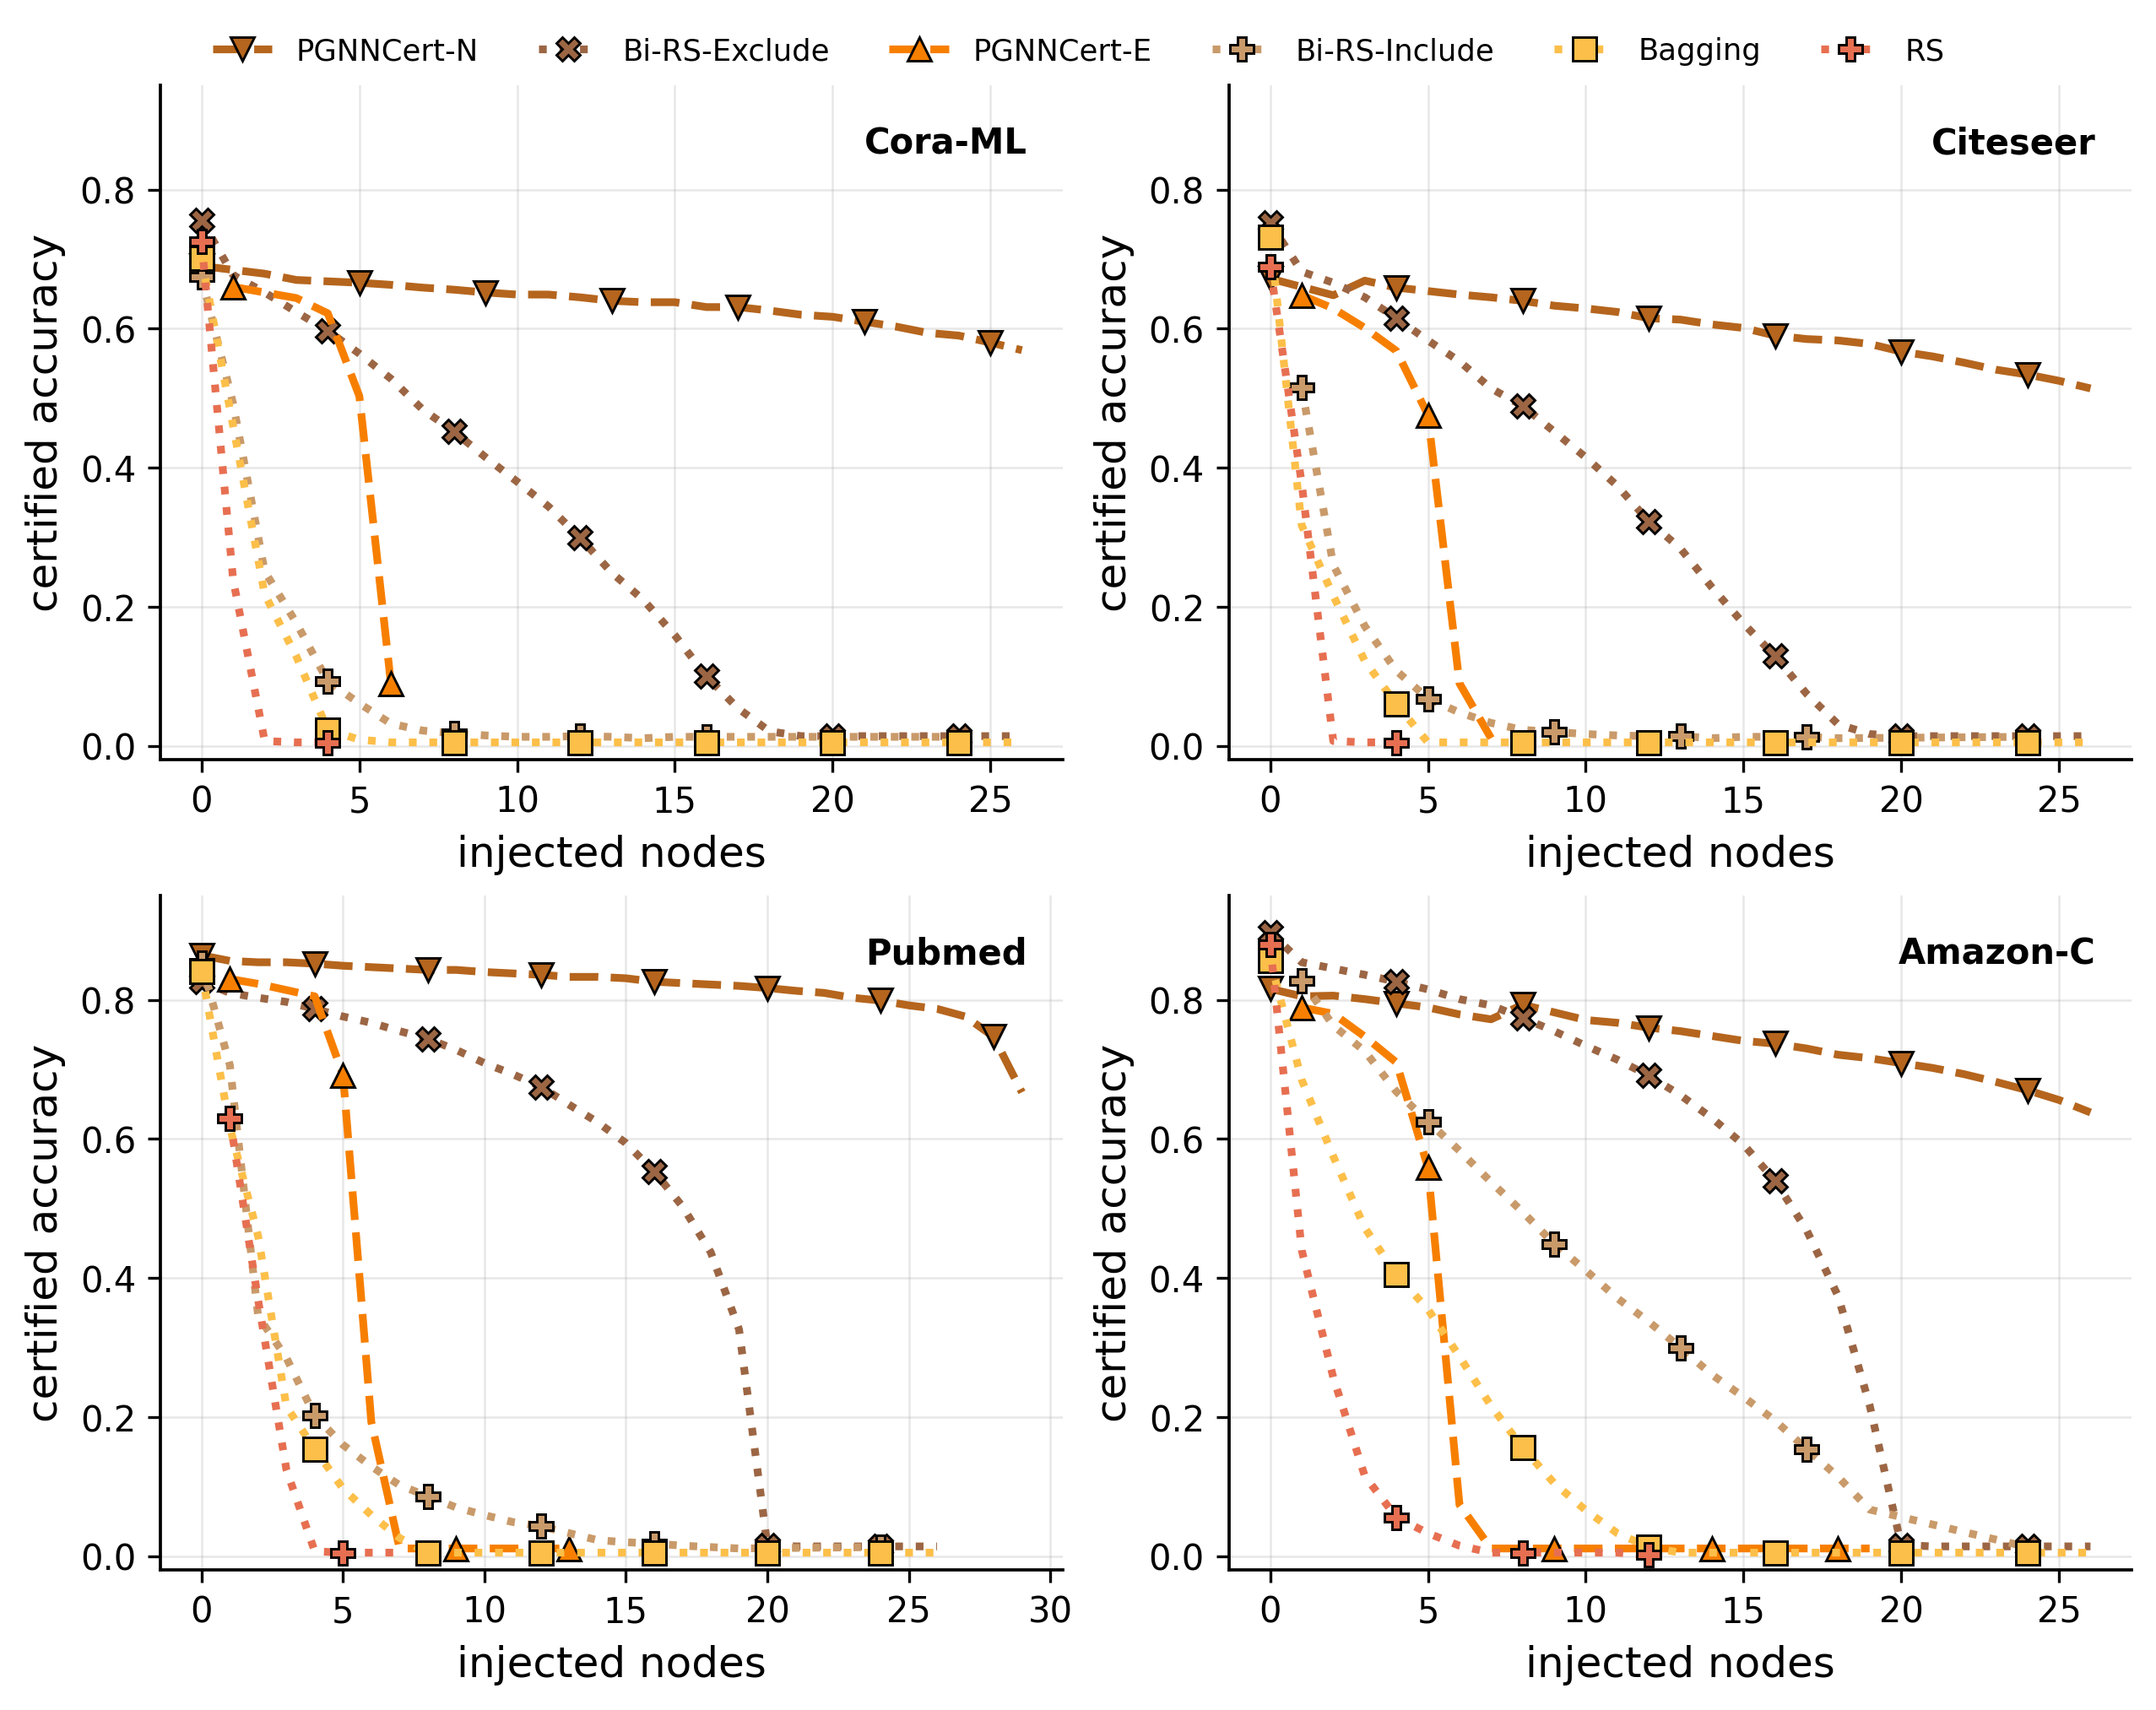
\includegraphics[width=\linewidth]{../../figures/F1b_node_injection_sota.png}
  \caption{Node-injection certified robustness across node datasets---a distinct
  threat model (node classification) shown as field context; \aeth{} targets
  graph-explanation edges.}
  \label{fig:nodeinj}
\end{figure}

\begin{table}[t]\centering
  \caption{Clean accuracy (5 seeds), \aeth{} vs.\ a plain GNN at the baseline's
  learning rate.}
  \label{tab:cleanacc}
  \begin{tabular}{lccc}
    \toprule
    Dataset & Base-GCN & \aeth{}-GCN & $\Delta$ \\
    \midrule
    AIDS & 0.986 & 0.989 & \win{$+0.3$} \\
    MUTAG & 0.762 & 0.769 & \win{$+0.7$} \\
    PROTEINS & 0.740 & 0.764 & \win{$+2.4$} \\
    DD & 0.725 & 0.758 & \win{$+3.4$} \\
    \midrule
    Cora-ML & 0.766 & 0.774 & $+0.8$ \\
    CiteSeer & 0.739 & 0.721 & \cav{$-1.7$} \\
    PubMed & 0.867 & 0.863 & $-0.4$ \\
    Amazon-C & 0.883 & 0.879 & $-0.3$ \\
    \bottomrule
  \end{tabular}
\end{table}

